\NewExpandableDocumentCommand{\TeXturedVERSION}{}{1.2.0}
%% Enable built-in LaTeX support for PDF/A compliance (must be before `\documentclass`)
\DocumentMetadata{lang=en, pdfversion=1.7, pdfstandard=A-2u}
%%% PDF/A compliance - glyph to Unicode mappings

%% NOTE: metadata are set up using the `hyperref` package in `preamble/general/hyperref.tex`

%% WARN: `pdfx` package is SUPERSEDED by built-in LaTeX support for PDF/A
%%       However, in case additional fonts are used, some glyphs may not be covered
%%       by default Unicode mappings, in which case they need to be mapped to Unicode
%%       code points manually (see below for GUIDE and examples).

%%% GUIDE: How to add missing unicode mappings for glyphs
%%
%% Consider following part of VeraPDF output for a non-compliant PDF:
%%   <rule specification="ISO 19005-2:2011" clause="6.2.11.7.2" testNumber="1" status="failed" passedChecks="0" failedChecks="1">
%%     <description>The Font dictionary of all fonts shall define the map of all used character codes to Unicode values,
%%                  either via a ToUnicode entry, or other mechanisms as defined in ISO 19005-2, 6.2.11.7.2.</description>
%%     <object>Glyph</object>
%%     <test>toUnicode != null</test>
%%     <check status="failed">
%%       <context>root/document[0]/pages[58](1323 0 obj PDPage)/contentStream[0](1324 0 obj PDContentStream)
%%                                          /operators[654]/usedGlyphs[0](RMTQUN+MSAM10 RMTQUN+MSAM10 57 0  0)</context>
%%       <errorMessage>The glyph can not be mapped to Unicode</errorMessage>
%%     </check>
%%   </rule>
%%
%% This means that some glyph on page 59 (indicated by a 0-based index `pages[58]`)
%% is missing a Unicode mapping. To fix this, we need to find the name of the glyph,
%% and provide a Unicode mapping for it. For further instructions how to proceed see
%% `preamble/pdfA-compliance/LaTeX-find-glyph-name/LaTeX-find-glyph-name.tex`.

\RequirePackage{iftex}
\ifluatex % only for luaLaTeX (sourced by default for pdfLaTeX)
    \RequirePackage{luatex85}
    %%% PDF/A compliance - glyph to Unicode mappings

%% NOTE: metadata are set up using the `hyperref` package in `preamble/general/hyperref.tex`

%% WARN: `pdfx` package is SUPERSEDED by built-in LaTeX support for PDF/A
%%       However, in case additional fonts are used, some glyphs may not be covered
%%       by default Unicode mappings, in which case they need to be mapped to Unicode
%%       code points manually (see below for GUIDE and examples).

%%% GUIDE: How to add missing unicode mappings for glyphs
%%
%% Consider following part of VeraPDF output for a non-compliant PDF:
%%   <rule specification="ISO 19005-2:2011" clause="6.2.11.7.2" testNumber="1" status="failed" passedChecks="0" failedChecks="1">
%%     <description>The Font dictionary of all fonts shall define the map of all used character codes to Unicode values,
%%                  either via a ToUnicode entry, or other mechanisms as defined in ISO 19005-2, 6.2.11.7.2.</description>
%%     <object>Glyph</object>
%%     <test>toUnicode != null</test>
%%     <check status="failed">
%%       <context>root/document[0]/pages[58](1323 0 obj PDPage)/contentStream[0](1324 0 obj PDContentStream)
%%                                          /operators[654]/usedGlyphs[0](RMTQUN+MSAM10 RMTQUN+MSAM10 57 0  0)</context>
%%       <errorMessage>The glyph can not be mapped to Unicode</errorMessage>
%%     </check>
%%   </rule>
%%
%% This means that some glyph on page 59 (indicated by a 0-based index `pages[58]`)
%% is missing a Unicode mapping. To fix this, we need to find the name of the glyph,
%% and provide a Unicode mapping for it. For further instructions how to proceed see
%% `preamble/pdfA-compliance/LaTeX-find-glyph-name/LaTeX-find-glyph-name.tex`.

\RequirePackage{iftex}
\ifluatex % only for luaLaTeX (sourced by default for pdfLaTeX)
    \RequirePackage{luatex85}
    %%% PDF/A compliance - glyph to Unicode mappings

%% NOTE: metadata are set up using the `hyperref` package in `preamble/general/hyperref.tex`

%% WARN: `pdfx` package is SUPERSEDED by built-in LaTeX support for PDF/A
%%       However, in case additional fonts are used, some glyphs may not be covered
%%       by default Unicode mappings, in which case they need to be mapped to Unicode
%%       code points manually (see below for GUIDE and examples).

%%% GUIDE: How to add missing unicode mappings for glyphs
%%
%% Consider following part of VeraPDF output for a non-compliant PDF:
%%   <rule specification="ISO 19005-2:2011" clause="6.2.11.7.2" testNumber="1" status="failed" passedChecks="0" failedChecks="1">
%%     <description>The Font dictionary of all fonts shall define the map of all used character codes to Unicode values,
%%                  either via a ToUnicode entry, or other mechanisms as defined in ISO 19005-2, 6.2.11.7.2.</description>
%%     <object>Glyph</object>
%%     <test>toUnicode != null</test>
%%     <check status="failed">
%%       <context>root/document[0]/pages[58](1323 0 obj PDPage)/contentStream[0](1324 0 obj PDContentStream)
%%                                          /operators[654]/usedGlyphs[0](RMTQUN+MSAM10 RMTQUN+MSAM10 57 0  0)</context>
%%       <errorMessage>The glyph can not be mapped to Unicode</errorMessage>
%%     </check>
%%   </rule>
%%
%% This means that some glyph on page 59 (indicated by a 0-based index `pages[58]`)
%% is missing a Unicode mapping. To fix this, we need to find the name of the glyph,
%% and provide a Unicode mapping for it. For further instructions how to proceed see
%% `preamble/pdfA-compliance/LaTeX-find-glyph-name/LaTeX-find-glyph-name.tex`.

\RequirePackage{iftex}
\ifluatex % only for luaLaTeX (sourced by default for pdfLaTeX)
    \RequirePackage{luatex85}
    \input{glyphtounicode.tex} % probably not loaded automatically for luatex
    \pdfgentounicode=1         % probably disabled by default for luatex
\fi

%% Enable in case some glyphs are missing from imported PDF figures
\pdfinclusioncopyfonts=1

%% Additional Unicode mappings for mathematical symbols (provided by `pdfx`)
%% https://gist.github.com/literalplus/045c4d090e2fe742157b4c903a984d24
\input{glyphtounicode-cmr.tex} % <- /usr/share/texmf-dist/tex/latex/pdfx/glyphtounicode-cmr.tex
% \input{glyphtounicode-ntx.tex} % <- /usr/share/texmf-dist/tex/latex/pdfx/glyphtounicode-ntx.tex


%%% Additional Unicode mappings for various extra glyphs

%% Glyphs: double brackets (of various sizes)
%% name of glyph found in /usr/share/texmf-dist/fonts/afm/public/stmaryrd/stmary5.afm
\pdfglyphtounicode{llbracket}{27E6} % https://codepoints.net/U+27E6
\pdfglyphtounicode{rrbracket}{27E7} % https://codepoints.net/U+27E7
\pdfglyphtounicode{largellbracket}{27E6 FE01} % variants according to size
\pdfglyphtounicode{largerrbracket}{27E7 FE01} % ... ... .. ....
\pdfglyphtounicode{Largellbracket}{27E6 FE02} % ... ... .. ....
\pdfglyphtounicode{Largerrbracket}{27E7 FE02} % ... ... .. ....
\pdfglyphtounicode{LARGEllbracket}{27E6 FE03} % ... ... .. ....
\pdfglyphtounicode{LARGErrbracket}{27E7 FE03} % ... ... .. ....
\pdfglyphtounicode{hugellbracket} {27E6 FE04} % ... ... .. ....
\pdfglyphtounicode{hugerrbracket} {27E7 FE04} % ... ... .. ....
\pdfglyphtounicode{Hugellbracket} {27E6 FE05} % ... ... .. ....
\pdfglyphtounicode{Hugerrbracket} {27E7 FE05} % ... ... .. ....
\pdfglyphtounicode{Hugellbrackettop}{23A5 23A1} % separate top, middle, bottom
\pdfglyphtounicode{Hugellbracketex} {23A5 23A2} % ... ... .. ....
\pdfglyphtounicode{Hugellbracketbot}{23A6 23A3} % ... ... .. ....
\pdfglyphtounicode{Hugerrbrackettop}{23A4 23A2} % ... ... .. ....
\pdfglyphtounicode{Hugerrbracketex} {23A5 23A2} % ... ... .. ....
\pdfglyphtounicode{Hugerrbracketbot}{23A6 23A2} % ... ... .. ....

%% Glyph: short minus
\pdfglyphtounicode{axisshort}{2212} % short minus -> minus https://codepoints.net/U+2212

%%% TODO: maybe use `\pdfstringdefDisableCommands` for something (in PDF metadata?)
 % probably not loaded automatically for luatex
    \pdfgentounicode=1         % probably disabled by default for luatex
\fi

%% Enable in case some glyphs are missing from imported PDF figures
\pdfinclusioncopyfonts=1

%% Additional Unicode mappings for mathematical symbols (provided by `pdfx`)
%% https://gist.github.com/literalplus/045c4d090e2fe742157b4c903a984d24
\input{glyphtounicode-cmr.tex} % <- /usr/share/texmf-dist/tex/latex/pdfx/glyphtounicode-cmr.tex
% \input{glyphtounicode-ntx.tex} % <- /usr/share/texmf-dist/tex/latex/pdfx/glyphtounicode-ntx.tex


%%% Additional Unicode mappings for various extra glyphs

%% Glyphs: double brackets (of various sizes)
%% name of glyph found in /usr/share/texmf-dist/fonts/afm/public/stmaryrd/stmary5.afm
\pdfglyphtounicode{llbracket}{27E6} % https://codepoints.net/U+27E6
\pdfglyphtounicode{rrbracket}{27E7} % https://codepoints.net/U+27E7
\pdfglyphtounicode{largellbracket}{27E6 FE01} % variants according to size
\pdfglyphtounicode{largerrbracket}{27E7 FE01} % ... ... .. ....
\pdfglyphtounicode{Largellbracket}{27E6 FE02} % ... ... .. ....
\pdfglyphtounicode{Largerrbracket}{27E7 FE02} % ... ... .. ....
\pdfglyphtounicode{LARGEllbracket}{27E6 FE03} % ... ... .. ....
\pdfglyphtounicode{LARGErrbracket}{27E7 FE03} % ... ... .. ....
\pdfglyphtounicode{hugellbracket} {27E6 FE04} % ... ... .. ....
\pdfglyphtounicode{hugerrbracket} {27E7 FE04} % ... ... .. ....
\pdfglyphtounicode{Hugellbracket} {27E6 FE05} % ... ... .. ....
\pdfglyphtounicode{Hugerrbracket} {27E7 FE05} % ... ... .. ....
\pdfglyphtounicode{Hugellbrackettop}{23A5 23A1} % separate top, middle, bottom
\pdfglyphtounicode{Hugellbracketex} {23A5 23A2} % ... ... .. ....
\pdfglyphtounicode{Hugellbracketbot}{23A6 23A3} % ... ... .. ....
\pdfglyphtounicode{Hugerrbrackettop}{23A4 23A2} % ... ... .. ....
\pdfglyphtounicode{Hugerrbracketex} {23A5 23A2} % ... ... .. ....
\pdfglyphtounicode{Hugerrbracketbot}{23A6 23A2} % ... ... .. ....

%% Glyph: short minus
\pdfglyphtounicode{axisshort}{2212} % short minus -> minus https://codepoints.net/U+2212

%%% TODO: maybe use `\pdfstringdefDisableCommands` for something (in PDF metadata?)
 % probably not loaded automatically for luatex
    \pdfgentounicode=1         % probably disabled by default for luatex
\fi

%% Enable in case some glyphs are missing from imported PDF figures
\pdfinclusioncopyfonts=1

%% Additional Unicode mappings for mathematical symbols (provided by `pdfx`)
%% https://gist.github.com/literalplus/045c4d090e2fe742157b4c903a984d24
\input{glyphtounicode-cmr.tex} % <- /usr/share/texmf-dist/tex/latex/pdfx/glyphtounicode-cmr.tex
% \input{glyphtounicode-ntx.tex} % <- /usr/share/texmf-dist/tex/latex/pdfx/glyphtounicode-ntx.tex


%%% Additional Unicode mappings for various extra glyphs

%% Glyphs: double brackets (of various sizes)
%% name of glyph found in /usr/share/texmf-dist/fonts/afm/public/stmaryrd/stmary5.afm
\pdfglyphtounicode{llbracket}{27E6} % https://codepoints.net/U+27E6
\pdfglyphtounicode{rrbracket}{27E7} % https://codepoints.net/U+27E7
\pdfglyphtounicode{largellbracket}{27E6 FE01} % variants according to size
\pdfglyphtounicode{largerrbracket}{27E7 FE01} % ... ... .. ....
\pdfglyphtounicode{Largellbracket}{27E6 FE02} % ... ... .. ....
\pdfglyphtounicode{Largerrbracket}{27E7 FE02} % ... ... .. ....
\pdfglyphtounicode{LARGEllbracket}{27E6 FE03} % ... ... .. ....
\pdfglyphtounicode{LARGErrbracket}{27E7 FE03} % ... ... .. ....
\pdfglyphtounicode{hugellbracket} {27E6 FE04} % ... ... .. ....
\pdfglyphtounicode{hugerrbracket} {27E7 FE04} % ... ... .. ....
\pdfglyphtounicode{Hugellbracket} {27E6 FE05} % ... ... .. ....
\pdfglyphtounicode{Hugerrbracket} {27E7 FE05} % ... ... .. ....
\pdfglyphtounicode{Hugellbrackettop}{23A5 23A1} % separate top, middle, bottom
\pdfglyphtounicode{Hugellbracketex} {23A5 23A2} % ... ... .. ....
\pdfglyphtounicode{Hugellbracketbot}{23A6 23A3} % ... ... .. ....
\pdfglyphtounicode{Hugerrbrackettop}{23A4 23A2} % ... ... .. ....
\pdfglyphtounicode{Hugerrbracketex} {23A5 23A2} % ... ... .. ....
\pdfglyphtounicode{Hugerrbracketbot}{23A6 23A2} % ... ... .. ....

%% Glyph: short minus
\pdfglyphtounicode{axisshort}{2212} % short minus -> minus https://codepoints.net/U+2212

%%% TODO: maybe use `\pdfstringdefDisableCommands` for something (in PDF metadata?)


\documentclass[12pt,a4paper]{report}

%% Set some toggle flags to control some of the document properties
%% Define some toggle flags

\newif\ifFANCY       %% whether to enable some more fancy stylistic choices
\newif\ifWIP         %% whether to enable debug commands, todos, etc.
\newif\ifEXTRAMARGIN %% whether WIP mode has extra right margin
\newif\ifCENSOR      %% whether to censor denoted passages

\FANCYtrue        %% by default, enable fancy features

% \FANCYfalse % disable some of the more fancy stylistic choices
%% NOTE: Comment out the following lines for the final version
\WIPtrue            % THIS IS A WORK-IN-PROGRESS VERSION
% \EXTRAMARGINtrue  % add extra right margin in WIP version (for notes/corrections)
% \CENSORtrue         % THIS IS A CENSORED VERSION

%% Preamble - data, packages, macros, and more
% \documentclass[draft, a4paper, english]{article}
\documentclass[a4paper, english]{article}

\usepackage{ifthen}
\newboolean{productionExport}
% \setboolean{productionExport}{true}
\setboolean{productionExport}{false}

\usepackage{graphicx} % Required for inserting images
\usepackage{hyperref}
\usepackage{glossaries}
\usepackage{paralist}
\usepackage{todonotes}
\usepackage{tcolorbox}
\usepackage{cleveref}
\usepackage{svg}
\usepackage[backend=biber,sortcites]{biblatex}
\setglossarystyle{altlist}

\usepackage{xcolor}
\newcommand{\tanke}[1]{\todo[color=teal]{{#1}}}
\newcommand{\info}[1]{\todo[color=green,nolist,fancyline]{{#1}}}
\newcommand{\hefe}{\textsc{Hefe}}

\setdefaultenum{(1)}{(a)}{i.}{A.}

\setlength\parindent{24pt}

\title{ \textsc{Masters essay}\\
\textit{Large Language Models Adaptation for Cyber-Physical System Testing}}
\author{Oliver Ruste Jahren\\
Department of Informatics\\
University of Oslo\\
\texttt{oliver.jahren@simulaacademy.no}}

\date{\today}

\addbibresource{refs.bib}

\makeglossaries
\newacronym{llm}{LLM}{Large Language Model}
\newacronym{llms}{LLMs}{Large Language Models}
\newacronym{ads}{ADSs}{Autonomous driving systems} 
\newacronym{ad}{ADS}{Autonomous driving system} 
\newacronym{jit}{JIT}{Just-In-Time} 
\newacronym{ml}{ML}{Machine learning} 
\newacronym{dl}{DL}{Deep learning} 
\newacronym{api}{API}{Application programming interface} 
\newacronym{apis}{APIs}{Application programming interfaces} 
\newacronym{csv}{CSV}{Comma separeted values} 
\newacronym{gui}{GUI}{Graphical user interface} 

\begin{document}
\maketitle

\ifthenelse{\boolean{productionExport}}{}{\listoftodos}
\chapter{Introduction}

% \epigraph{The whole is greater than the sum of its parts.}{Aristotle}

\section{Motivation}

\textbf{Conventional cars} are ubiquitous in society. Whether for freight trafficking or for humans, cars have great flexibility with their ability to go wherever without requiring tailored infrastructure
such as railway tracks. They do, however, have one major weak point --- the human driver. For this
reason, industry and academia have put forward efforts to enhancing cars with \acrfull{ads}
capabilities.
By \textbf{empowering humans} with autonomous vehicles, it is expected that traffic efficiency will
increase and road fatalities will fall.

\textbf{Due to the critical safety situation of manoeuvring a car} In a public setting where other external
actors are present, it is essential that \acrlongpl{ads} are thoroughly tested before they are
deployed so that they are confirmed to be sufficiently safe and capable of handling the situations in which
they may typically end up.
But due to the complicated nature of the typical \acrshort{ads} operating environment, coming up with
exhaustive system test solutions is near impossible.
For this reason we want a way of testing the system that is capable of pushing the \acrlong{ads} to
its limits such that we can measure its performance and see if it is capable of
handling complex scenarios.

\textbf{Having an existing repository of \acrlong{ads} test cases,} such as
DeepScenario we wish to improve them. \textbf{\acrfullpl{llm}} have demonstrated
great capabilities of context learning and emergent abilities, which begs
the question of their  applicability for \acrshort{ads} testing.  There are
various methods of testing  \acrlong{ads}. Can these existing test methods be
improved by applying \acrshort{llm} technology to them?

% Yet, testing is \textit{important} for \acrlong{ads}, and text case generation is costly. We
% therefore pose the question: Can \acrshort{llms} be applied for (1) lowering the
% cost of testing, and (2) increasing the thouroughness of \acrlong{ads} testing?

\newpage % Legger inn en ny side siden thesis overview uansett konsumerer den siden

\section{Research questions}

TODO: formalize research questions.

\section{Thesis overview}

The thesis is structured as follows:

\begin{itemize}
    \item \Cref{sec:background} introduces key concepts related to \acrshortpl{ads} and \acrshortpl{llm}.
    \item \Cref{sec:problemDescription} defines the specific problem addressed in this work.
    \item \Cref{sec:literatureReview} reviews the current state of research in the field.
    \item \Cref{sec:relatedWork} discusses related applied works and lessons learned.
    \item \Cref{sec:solutionProposal} details our proposed solution and its technical aspects.
    \item \Cref{sec:experiments} describes the experimental setup used to evaluate the solution.
    \item \Cref{sec:results} presents the findings from the experiments.
    \item \Cref{sec:discussion} analyzes and compares the results to existing work.
    \item \Cref{sec:furtherWork} suggests directions for future research.
    \item \Cref{sec:conclusion} summarizes the main contributions and findings.
\end{itemize}

Two appendices are included: \Nref{sec:fileDiffs} and \Nref{sec:errorMessages}.

\ifthenelse{\boolean{productionExport}}{\newpage}{}
% \newpage
\tableofcontents
\listoffigures

\iftrue
    \setlength\parindent{0pt}
    \setlength{\headsep}{5pt}
    \setlength{\parskip}{1em}
\fi

% \newpage

\ifthenelse{\boolean{productionExport}}{\newpage}{}
\chapter{Background}

\epigraph{The limits of my language mean the limits of my world}{Wittgenstein}

\section{Testing}

First, we need to establish some basic testing concepts.

\subsection{Pre- and post-conditions}\label{sec:testingConditions}

When running test cases, the concept of \textit{Pre-conditions}
refers to certain properties that
obtain \textit{before} running a given test case. E.g that the \acrshort{ads} ego vehicle is
stationary.

In many ways mirroring pre-conditions, \textit{post-conditions} refers to the properties that obtain
\textit{after} having ran a test. E.g. that the ego vehicle will be moving after having performed
the test.

% TODO: The testing conditons should ideally be cited.

\subsection{Test coverage}\label{sec:testCoverage}

\textbf{Test coverage} refers to the what degree the entire system is being tested. The concept can
be used to describe both hardware and software test
coverage~\cite[187]{testCoverage94}.~\citeauthor{testCoverage94} posit that hardware-based test
coverage is measured in terms of the number of possible faults covered, whereas software-based test
coverage is measured in terms of the amount of structural or data-flow units that have been
exercised~\cite[187]{testCoverage94}. A test case that exercised every single code line of the
system would by definition have perfect test coverage.


% \subsection{Autonomous systems}
% 
% Autonomous systems are systems that are capable of changing their behaviour in
% response to unanticipated events during
% operation~\cite[368]{watson2005autonomous}. Autonomous systems exist in several
% different forms and they are typically tailored for their specific operating
% environments. Some systems operate in the maritime domain, some in the air, and
% others on the ground in the terrestrial operating domain~\cite[369-370]{watson2005autonomous}.

\section{\acrfullpl{ads}}

\acrfull{ads} are systems that enable automotive vehicles to drive autonomously. Due to the typical
operating scenarios of a car it is pivotal that the \acrlong{ads} maintain a high safety standard. A
common way to assert safety is to use simulator based testing~\cite[1]{DeepScenario}.

\subsection{\acrlong{ads} testing}

Testing is essential for assuring \acrlong{ads} operative safety~\cite[163]{ADTestingReview16}.
Several methods for testing exist, testing various aspects of the \acrlong{ads}. An \acrshort{ads}
typically exists of several modules, all working together and handling different aspect of the
\acrlong{ads}.

\citeauthor{ADTestingReview16} outline several typical architectures for \acrshort{ads} testing,
drawing on traditional software testing traditions outlining how \textit{software testing} can be
used alongside more specialized \acrshort{ads} testing techniques such as \textit{simulation
    testing} and \textit{X-in-the-loop testing}~\cite[163-164]{ADTestingReview16}.

\subsection{\acrlong{ads} driveability}\label{sec:adsDrivability}

\textbf{Driveability} is a high-level estimator of the overall driving
condition of an \acrshort{ads}, derived from several lower-level sources~\cite[3140]{safeToDrive}.
It can be used to refer to various aspects of a scene.
\citeauthor{safeToDrive} discuss the concept further, using the  scene definition
of~\citeauthor{scenes} as outlined in  \Cref{sec:adsSimConcepts}, they describe
how driveability can refer both to \begin{inparaenum}
    \item road conditions, and
    \item human driver performance.
\end{inparaenum}
\citeauthor{safeToDrive} go on to give an overview of how driveability
can be used to refer to a \begin{inparaenum}\setcounter{enumi}{2}
    \item \textit{driveability map} which divides a map into
    cells indicating where the \acrshort{ads} expects that it will be able to go, and
    \item \textit{object driveability}, which refers to the classification of physical objects in
    the environment that the \acrshort{ads} expects that it can run over without causing damage to
    the ego vehicle~\cite[3135-3136]{safeToDrive}.
\end{inparaenum}

The main method for assessing the driveability of a scene comes form assessing the environment of
the scene. Factors such as \begin{inparaenum}
    \item weather,
    \item traffic flow,
    \item road condition, and
    \item obstacles \end{inparaenum} all play into this. The \acrshort{ads} infers information from
observation~\cite[3136]{safeToDrive}.

They continue to give an overview of various \textit{driveability factors} and their associated
difficulties, using a a split between \textit{explicit} and \textit{implicit} factors.

\textbf{Explicit driveability factors} will typically include factors such as \textbf{Extreme
    weather} such as \begin{inparaenum}
    \item fog,
    \item heavy rain,
    \item snow,
\end{inparaenum}
all serving to impair road visibility and causing increased difficulties for vision-based tasks such
as road detection and object tracking~\cite[3136-3137]{safeToDrive}. \textbf{Illumination} also
poses various challenges for typical \acrshort{ads} tasks as a typical \acrshort{ads} will be
required to operate in a plethora of scenes with varying degrees of illumination depending on
factors such as time of day and location (e.g. if the \acrshort{ads} is operation in a dimly lit
tunnel)~\cite[3137]{safeToDrive}. The authors highlight how low illumination may serve as an
advantage for the \acrshort{ads} as this allows for using the head lights of other vehicles as a
feature for detecting them, whereas it make pedestrian detection significantly more
challenging~\cite[3137]{safeToDrive}. \textbf{Road geometry} is another external factor, satisfying
our natural intuition that \textit{intersections} and \textit{roundabouts} are more difficult to
drive through than straight highways~\cite[3137]{safeToDrive}.

\textbf{Implicit driveability factors} consist of behaviours and intent of other road users
interacting with the autonomous car~\cite[3138]{safeToDrive}. This includes the actions of other
vehicles such as their \begin{inparaenum}
    \item overtaking,
    \item lane changing,
    \item rear-ending,
    \item speeding, and
    \item failure to obey traffic laws \end{inparaenum}.~\citeauthor{safeToDrive} call these factors
\textbf{vehicle behaviours}~\cite[3138]{safeToDrive}. Furthermore, \textbf{pedestrian behaviours}
are also taken into account, noting how pedestrians can sometimes
\begin{inparaenum}\setcounter{enumi}{5}
    \item cross the road,
    \item be inattentive, or
    \item fail to comply with the traffic law \end{inparaenum}\cite[3138]{safeToDrive}. They go on
to describe the \textbf{driver behaviour} of other drivers pointing out how
\begin{inparaenum}\setcounter{enumi}{8}
    \item distraction, and
    \item drowsiness \end{inparaenum} can be factors that cause accidents even for
\acrshort{ads}-enhanced vehicles due to the other, manual, cars
interfering with their operation~\cite[3138-3139]{safeToDrive}. Lastly
\textbf{motorcyclist/bicyclist behaviours} cause their own source of implicit driveability factors:
The models and methods developed for analysing the group's behaviour are far more limited than other
groups of road users~\cite[3139]{safeToDrive}.~\citeauthor{safeToDrive} theorise that this comes
down to the lack of available datasets that capture and label the trajectories and behaviours
of motorcyclists and bicyclists~\cite[3139]{safeToDrive}, causing potential issues for any
\acrshort{ads} that wishes to operate in a shared traffic environment with this group.

\subsection{\acrlong{ads} testing metrics}\label{sec:adsMetrics}

When evaluating \acrshort{ads} testing, several metrics can be used. What metric to use will depend
on what the relevant test is measuring.

Building on what we have learnt about driveability (\Cref{sec:adsDrivability}),
we take after \citeauthor{safeToDrive} and review three metrics for
quantifying driveability: \begin{inparaenum}
    \item scene driveability,
    \item collision-based risk, and
    \item behaviour-based risk.
\end{inparaenum}

\textbf{Scene driveability} refers to how easy a scene is for an
\acrshort{ads} to navigate, and the \textit{scene driveability score} refers to
how likely the \acrlong{ads} is to fail at traversing the
scene~\cite[3140]{safeToDrive}. It is typically found through and end-to-end
approach. Note how this is a metric for \textit{scenes}, without taking into
account the performance of any specific \acrshort{ads}.

\textbf{Collision-based risk} comes in two kinds - \begin{inparaenum}
    \item binary risk indicator, and
    \item probabilistic risk indicator.
\end{inparaenum} \citeauthor{safeToDrive} posit that the prior, binary metric, indicates whether a
collision will happen in the near future in a binary `either-or' sense, whereas the latter yields a
probability calculated based on current states, event, choice of hypothesis, future states and
damage~\cite[3140]{safeToDrive}.

\textbf{Behaviour-based risk} estimation also represents a binary classification problem wherein
nominal behaviours are learnt from data, and then dangerous behaviours are detected on that. This
requires a definition of `nominal behaviour', which is typically defined on on acceptable speeds,
traffic roles, location semantics, weather conditions and/or the level of fatigue of the
driver~\cite[3140]{safeToDrive}. Furthermore \citeauthor{safeToDrive} describe how this metric also
allows more than one \acrshort{ads} to be labelled as `conflicting' or `not
conflicting'~\cite[3140]{safeToDrive}, representing a ruling on their compatibility. Finally, they
note how behaviour-based risk assessment typically focuses on driver behaviours, not taking into
account other actors in the scene such as pedestrians or cyclists.

\subsection{The complexities of \acrshort{ads} testing}\label{sec:adsTestingComplexity}

As we have seen, \acrshortpl{ads} can perform several tasks, in several environments. As such, there
are several relevant factors for testing them. It is not feasible to test all potential variations
of all potential environments in the real world, meaning that the \textit{test
    coverage}\footnote{See \Nref{sec:testCoverage}} typically will be low.

Some of the factors that complicate \acrshort{ads} operations are \begin{inparaenum}
    \item timing,
    \item sequence of events, and
    \item parameter settings such as the different speeds of various vehicles and other actors.
\end{inparaenum}

\citeauthor{adsComplexityIndex18} posit that \textit{the concept of complexity exists everywhere,
    but there is no agreement on one for driving situations}~\cite[1182]{adsComplexityIndex18}.
Therefore they introduce their own concept of \acrfull{dsc}, which serves to give a metric of a
the complexity of a given driving situation. Their \acrshort{dsc} is defined as the output of a
mathematical formula taking into account the perplexity and standard deviation of several
control variables $\mathcal{M}$ representing the surrounding vehicle's
behaviour~\cite[1182]{adsComplexityIndex18}. Their formula also takes into account the ratio of
\textit{V2X}-capable vehicles~\cite[1182]{adsComplexityIndex18}, i.e. the vehicles that are
connected and capable of communicating~\cite[1]{v2xTestingSurvey2019}.

% It is common to modularize the testing of \acrshort{ads} so that the individual modules can be
% tested in isolation. The modules of an \acrshort{ads} typically include a motion planner, a
% \acrfull{cv} system, and % LIDAR. This allows for testing the individual modules in a way that
% makes sense for their specific domains.

\subsection{\acrlong{ads} simulation}

Due to the complexity involved in testing \acrlongpl{ads} (\Cref{sec:adsTestingComplexity}),
simulators are typically used for this purpose~\cite{DeepScenario}. While the same points about not
being able to test \textit{all} possible scenarios do remain true for simulator based testing due to
the sheer number of factors, using a simulator allows for far greater testing at far lower cost due
to the minimal overhead of
\begin{inparaenum}
    \item generating,
    \item running, and
    \item evaluating the outcome of
\end{inparaenum}
test cases.

Furthermore, simulators allow for greater flexibility in determining the test scenarios due to not
being confined by the  physical world that is available to the scientist that wishes to perform the
testing. Using a simulator, a Europe-based scientist can test their \acrshort{ads} for North
American conditions, or vice-versa.

\subsection{The \acrshort{ads} simulator jungle}\label{sec:simulatorOverview}

Due to the appeal of running \acrshort{ads} simulation, several contenders exist
on the market.

\textbf{Carla} is a widely used \acrshort{ads} simulator~\cite{Carla}. It is implemented
using the game engine UnrealEngine~\cite{unrealengine} and allows for running
test cases under various scenarios and collecting their results. Carla is fully
open source and is under active development. It has been applied in projects such as KITTI-Carla,
which generated a KITTI dataset using Carla~\cite{kittiCarla}.

\textbf{LGSVL} is a deprecated simulator from LG~\cite{lgsvl}. It was used in projects such
as DeepScenario~\cite{DeepScenario}. It allowed for running various maps with various vehicles and
tracking their data. It was also capable of generating HD
maps \footnote{\url{https://github.com/lgsvl/simulator?tab=readme-ov-file\#introduction}}.
DeepScenario is a project similar to this, concerned with testing \acrlongpl{ads}. Further details
about it in are located in \Nref{sec:relatedWork}.

\textbf{AirSim} is Microsoft's offering~\cite{airsim}. It has, like LGSVL,
been deprecated. It is also built using UnrealEngine. Unlike the other
simulators we have seen, this also focused on autonomous vehicles outside of
only cars, such as drones.


\subsection{Concepts of \acrshort{ads} simulation}\label{sec:adsSimConcepts}

\citeauthor{scenes} draw up an outline for the terms \textit{scene}, \textit{situation}, and
\textit{scenario}, that are all concepts widely used in \acrshort{ads} simulation testing.

\textbf{scene} is a term that is used in different manners in various
articles~\cite[982]{scenes}, but \citeauthor{scenes} propose standardising the definition on
\textit{a scene describing a snapshot of the environment including the scenery and dynamic elements,
    as well as  as all actors’ and observers’ self-representations, and the relationships among those entities}~\cite[983]{scenes}.

\textbf{situation} is, like \textit{scene}, employed in various fashions. \citeauthor{scenes}
give a background detailing its usage ranging from \textit{"the entirety of circumstances,
    which are to be considered by a robot for its selection of an appropriate behaviour pattern in a
    particular moment'}\footnote{The translation from German is borrowed from \citeauthor{scenes},
    \cite[984]{scenes}}, in  \citeauthor{scenarioTysk}~\cite[3]{scenarioTysk} to
\citeauthor{schmidtScenario} introducing a distinction between \textit{the true world} in a formal
sense, and that being the ground truth upon which a situation is
described~\cite[892]{schmidtScenario}.

\citeauthor{scenes} propose to standardise on the definition of a situation being \textit{
    the entirety of circumstances, which  are to be considered for the selection of an
    appropriate behaviour pattern at a particular point of time}~\cite[985]{scenes}.

\textbf{scenario} refers to \textit{'the temporal development between several scenes in a sequence
    of scenes'}\cite[986]{scenes}. We note how the definition a a scenario utilises that of a scene.
Furthermore, \citeauthor{scenes} hold it to be the case that \textit{'every scenario starts with an
    initial scene. Actions \& events as well as goals \& values may be  specified to characterize
    this temporal development in a scenario'}~\cite[986]{scenes}, clarifying the distinction
between a scenario and a scene.

Lastly they posit that a scenario spans a certain amount of time, whereas a scene has no such
temporal aspect to it.


When running a simulation, we refer to the autonomous vehicle that is being
simulated as the \textit{ego vehicle}~\cite{egoDefinition}.

% introduce the concept of a \textit{scene}, which denotes 

% An alternate simulator is LG SVL~\cite{lgsvl}, but it has been deprecated since
% 2022 and as such it does not seem proper to build a new solution on top of it.
% The DeepScenario dataset~\cite{DeepScenario} utilises this simulator framework.
% \tanke{The LGSVL part can be removed - not relevant?}

\subsubsection{\acrshort{ads} scenario formats}\label{sec:adsScenarioFormats}

\textbf{OpenSCENARIO} is a standard developed by the Association for Automation and
Measurement Systems (ASAM), which is dedicated to the description of dynamic
scenarios~\cite[651]{generatingOpenScenario}. Under this format, only the
\textit{dynamic} content of the scenario is recorded in the file. The static
content is kept in other formats such as OpenDRIVER and
OpenCRG~\cite[652]{generatingOpenScenario}. The simulator Carla (outlined in
\Cref{sec:simulatorOverview}) supports this
standard~\cite[652]{generatingOpenScenario}.

Another widely popular scenario format is
\textbf{CommonRoad}~\cite[4941]{convOpenScenarioToCR}, first proposed in
\citedate{commonRoadOG}~\cite{commonRoadOG}. There are tools such as those
proposed by \citeauthor{convOpenScenarioToCR} that allows for converting
OpenSCENARIO scenarios to the CommonRoad
format~\cite[4941]{convOpenScenarioToCR}.

% TODO: Skrive om Carlas støtte for Python-scenarioer
% TODO: Skrive om Carla scenario runner her?

\section{\acrfullpl{llm}}

\acrfullpl{llm} are transformer-based language models that typically contain several hundred billion
parameters and are trained on massive text data~\cite[4]{llmSurvey}.
Base language models, as the name implies, \textit{model language}. They are typically statistical
models and an example of \acrfull{ml}.

\subsection{\acrfull{llm} architecture}\label{sec:llmArch}

A \acrlong{llm} is a neural network trained on big data~\cite[3]{llmSurvey}. They expand on the
older statistical language models by training on more data. This gives rise to \textit{emerging
    abilities} such as in context learning~\cite[3]{llmSurvey} (\Nref{sec:emergentAbilities}). These
older statistical models are also neural networks, but they were impractical to train on large
amounts of data. It was not until the seminal paper \textsc{Attention is all you
    need}~\cite{attentionIsAllYouNeed} that a Google team headed by~\citeauthor{attentionIsAllYouNeed}
showed how neural networks can be trained in parallel using their new \textit{attention} mechanism.
This allowed for using amounts of data that was not technologically practical up until that point,
opening the door for later advancements such as
ChatGPT~\cite[9]{llmSurvey}

% \todo{Should elaborate further?}
\citeauthor{jm} describe how \acrshortpl{llm} rely on \textit{pretraining}.

\subsubsection{The importance of training data}

As a consequence of \acrshortpl{llm} being statistical models of a certain input
data~\cite[1]{llmSurvey}, what data the model is trained on is of great
importance for the capabilities of the model~\cite[6]{llmSurvey}.
\citeauthor{llmSurvey} give an overview of various \acrshortpl{llm} and what
kinds of corpora\footnote{A corpus (pl. corpora) refers to a document
    collection.} they have been trained on~\cite[11-14]{llmSurvey}.

The training data will provide the model with its base understanding of the
world, and as such it will dictate \begin{inparaenum}
    \item what it `knows', and
    \item how we should interact with it.
\end{inparaenum}
E.g., if we want to solve problems related to software code, we should employ a
model that has been \textit{trained} on software code related topics so that the
probability of it predicting correct tokens will be higher. If it has not seen
any code during its training it would not have any base `knowledge' for solving
our problem, and its output would be bad. The \acrshort{llm} would however have
no way of knowing if its output would be right or wrong, and we could say that
it would have \textit{hallucinated}.
See \Nref{sec:llmProblems} for further information
about hallucination.


\subsection{Emergent abilities}\label{sec:emergentAbilities}

\citeauthor{emergentabilitiesLLM} outline how \textit{emergent abilities} appear
when scaling up language models~\cite[1]{emergentabilitiesLLM}. They define
\textit{emergent ability} to refer to abilities that are not present in smaller
models, but present in the larger ones\cite[1]{emergentabilitiesLLM}, building
on physicist~\citeauthor{anderson1972more} stating that \textit{Emergence is
    when quantitative changes in a system result in qualitative changes in
    behaviour.}~\cite[2]{emergentabilitiesLLM}.

Furthermore, they discuss how \textit{few-shot prompting} typically can achieve
far superior results for harvesting \acrshort{llm} emergent abilities, whereas
one-shot prompting can perform worse than randomized
results~\cite[3-4]{emergentabilitiesLLM}.

They continue outlining several approaches for achieving augmented prompting
strategies, underlining how \begin{inparaenum}
    \item multi-step reasoning
    \item instruction following
    \item program execution,
    and
    \item model calibration
\end{inparaenum}
all serve as possible ways of increasing \acrshort{llm} performance~\cite[5]{emergentabilitiesLLM}.

% \tanke{Burde bygge på forrige seksjon om "små" language models}

\subsection{Intelligence in \acrshortpl{llm}}\label{sec:llmIntelligence}

There are three theories on machine intelligence, each serving to
explain how they `\textit{think}': \begin{inparaenum}
    \item stochastic parrot
    \item Sapir-Whorf hypothesis,
    and
    \item conceptual blending.
\end{inparaenum}

\subsubsection{Stochastic parrot}\label{sec:llmParrot}

\citeauthor{parrot} outline how \acrshortpl{llm} can \textit{fool} humans as they
are trained on ever larger amounts of parameters and data, appearing to be in possession of an
intelligence~\cite[610-611]{parrot}.

This anticipates the phenomenon of hallucination (\Cref{sec:llmHallucination}).

\subsubsection{Sapir-Whorf hypothesis}

The Sapir-Whorf hypothesis posits that  \textit{The structure of anyone’s native
    language strongly influences or fully determines the world-view he will acquire
    as he learns the language.}~\cite[128]{sapirWhorf}.

We note how this maps to our \acrshortpl{llm}, indicating that they will only ever
be able to `know' the data on which they have come into contact with.

Or: \textbf{Language} defines the possible room for \textbf{thought}.


\subsubsection{Conceptual blending}
%Relevant?

Conceptual blending is a theory on intelligence. It refers to the basic mental
operation that leads to new meaning or insight that occurs when one identifies
a match between to input mental spaces, to project selectively from those inputs
into a new `blended' mental space~\cite[57-58]{conceptBlending}.

This phenomenon explains how we are able to imagine phenomena that logically
should not exist such as \textit{land yacht} (\Nref{fig:landYacht})

\begin{figure}[h]
    \centering
    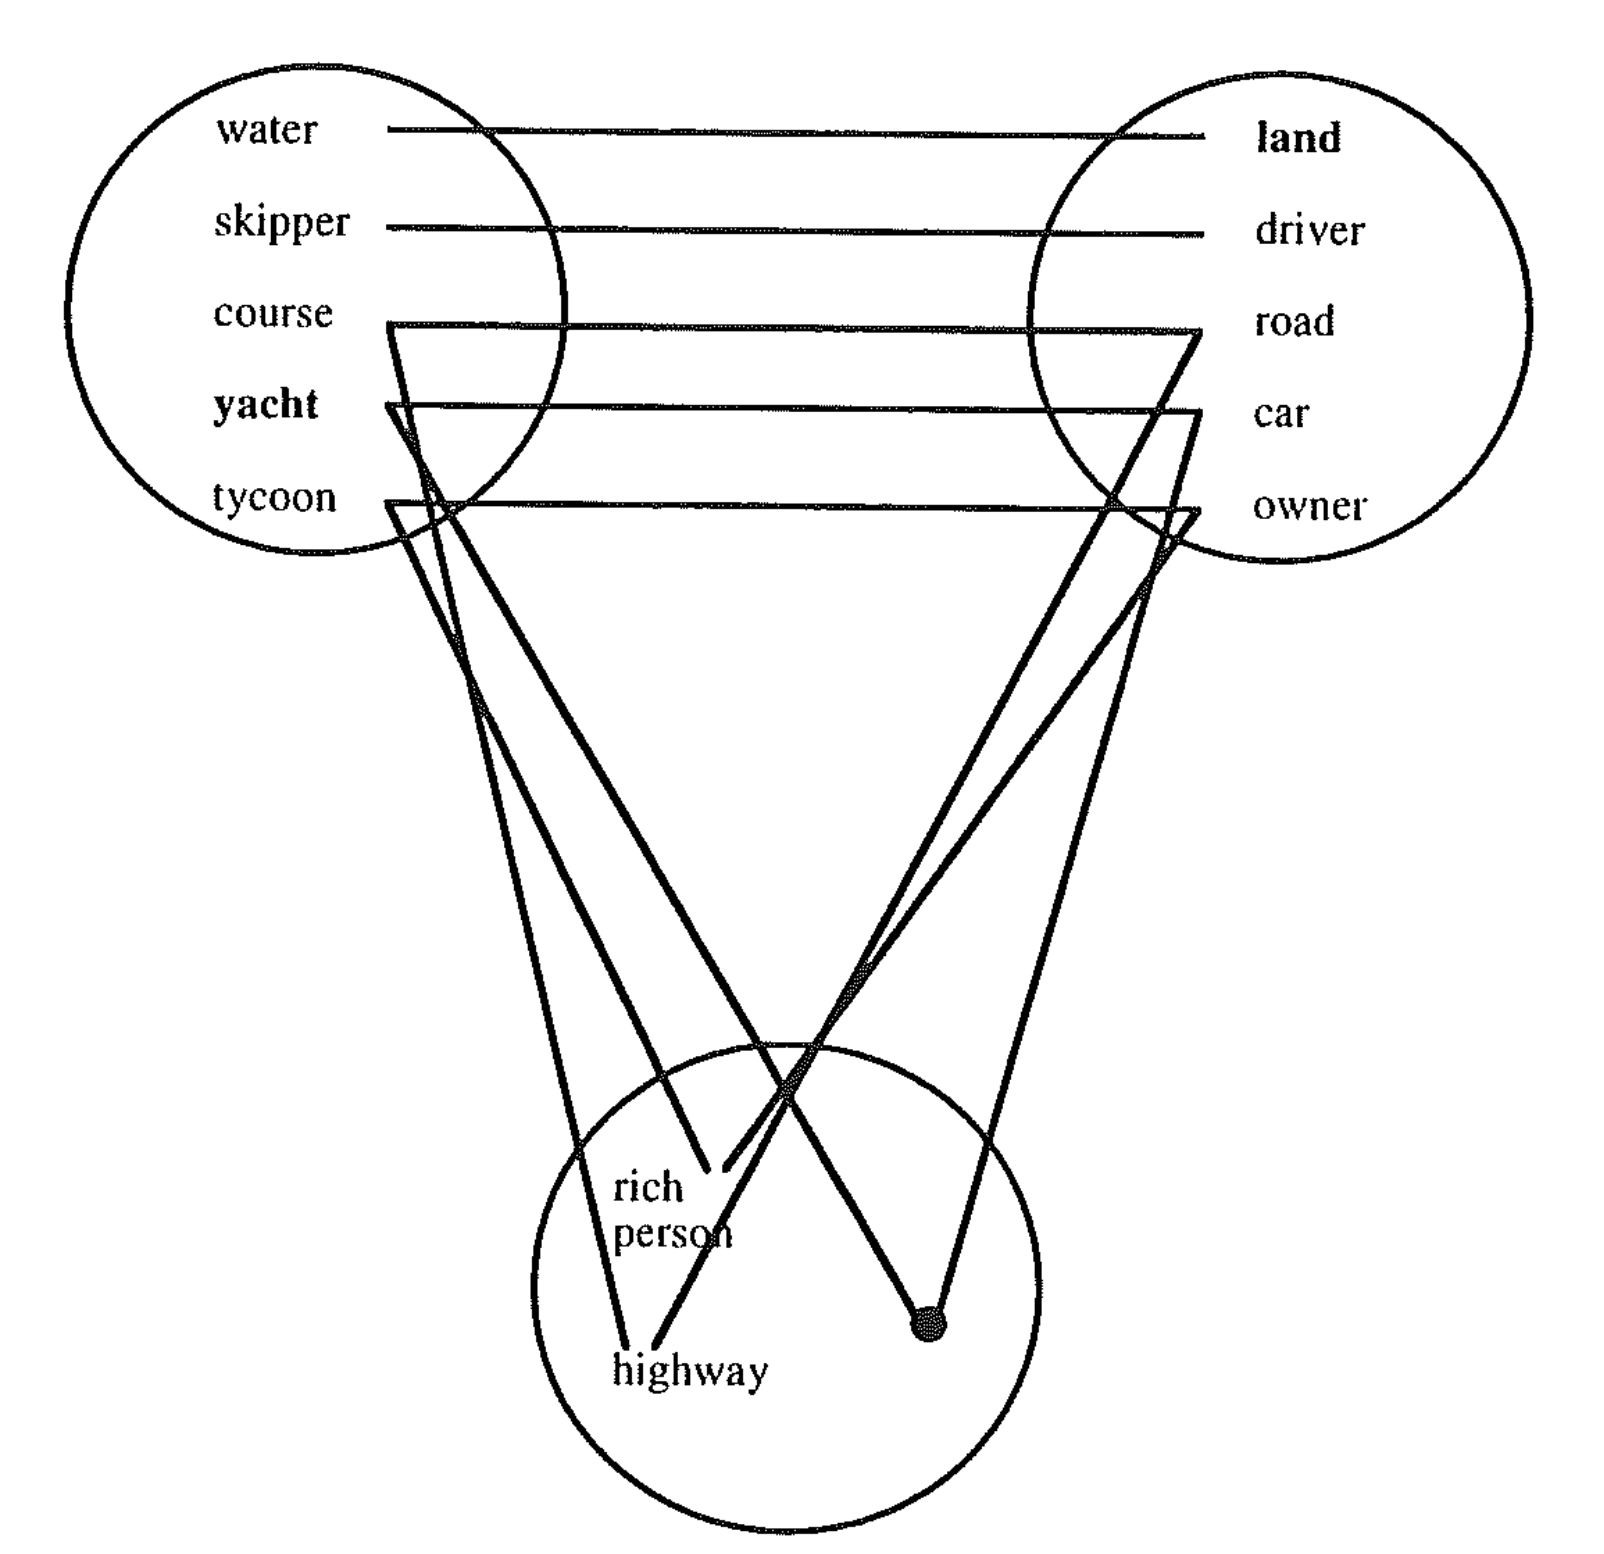
\includegraphics[width=0.8\textwidth]{figures/landYacht.png}
    \caption[Land yacht conceptual blend]{The conceptual blend of a \textit{land
            yacht}\footnotemark}\label{fig:landYacht}
\end{figure}

\footnotetext{Diagram borrowed from \citeauthor{conceptBlending},~\cite[67]{conceptBlending}.}

We note how this is how \acrshortpl{llm} operate when processing vectorized
linguistic data.
% Conceptual blending is a theory on both machine and human intelligence. 


\subsection{Utilising \acrshortpl{llm} - Prompt engineering}\label{sec:llmUtilization}


A typical way of interacting with \acrshortpl{llm} is \textit{prompting}~\cite[44]{llmSurvey}. You
prompt the model to solve various tasks. As we saw in \Nref{sec:emergentAbilities}, the level of
performance you are able to extract from your \acrlong{llm} can depend a great deal on how you
interact with it. The process of manually creating a suitable prompt is called \textbf{prompt
    engineering}~\cite[44]{llmSurvey}.~\citeauthor{llmSurvey} outline three principal prompting
approaches:

\textbf{\acrfull{icl}} is a representative prompting method that formulates the task
description and/or demonstrations in natural language text~\cite[44]{llmSurvey}. It is based on
\textit{tuning-free prompting} and it, as the name implies, never tunes the parameters of the
\acrshort{llm}~\cite[15]{promptingSurvey}. One the one hand, this allows for efficiency, but on the
other hand, heavy engineering is typically required to achieve high accuracy, meaning you must
provide the \acrshort{llm} with several answered prompts~\cite[16]{promptingSurvey}. In layman's
terms, \acrshort{icl} entails including examples of the process you want the model to perform when
prompting it.

\textbf{\acrfull{cot} prompting} is proposed to enhance \acrlong{icl} by involving a
series of intermediate reasoning steps in prompts~\cite[44, 52]{llmSurvey}. The basic concept of
\acrshort{cot} prompting, is including an actual \acrlong{cot} inside the prompt that shows the way
form the input to the output~\cite[52]{llmSurvey}.~\citeauthor{llmSurvey} note that the same effect
can be achieved by including simple instructions like `\textit{Let's think step by step}' and other
similar `magic prompts' in the prompt to the \acrshort{llm}, making \acrshort{cot} prompting easy to
use~\cite[52]{llmSurvey}.

\textbf{Planning} is proposed for solving complex tasks, which first breaks them down into smaller
sub-tasks and then generates a plan of action to solve the sub-tasks one by
one~\cite[44, 54]{llmSurvey}. The plans are being generated by the \acrshort{llm} itself upon
prompting it, and there is a distinction between text-based and code-based approaches. Text-based
approaches utilise natural language, whereas code-based approaches utilise executable computer code~\cite[54-55]{llmSurvey}.


\subsection{General challenges with \acrshortpl{llm}}\label{sec:llmProblems}

We have seen that \acrshortpl{llm} demonstrate promising abilities (\Nref{sec:emergentAbilities}) But they have nevertheless certain issues attached to them that we need to be aware of.

\subsubsection{Hallucination}\label{sec:llmHallucination}

As we saw in \Cref{sec:llmParrot}, \acrshortpl{llm} are prone to
\textit{bullshitting}. They have no intuition of, or concern with \textit{the
    truth}. They only ever yield whatever response is the most probable under their
\textsc{beam search} algorithm being applied on their training data.

\subsubsection{Environmental concerns}

A University of Rhode Island study on the environmental impact of \acrshortpl{llm} have shown that
they require wast amount of energy and water~\cite{hungryLlm}. They also found that the different
\acrshortpl{llm} may differ greatly in their energy consumption, highlighting that that certain
\acrshortpl{llm} may consume more than \num{70} times more energy than others~\cite{hungryLlm}.

Another study by \citeauthor{llmCarbon} focusing specifically on \textit{carbon emissions} did
however find that these emissions significantly lower for \acrshortpl{llm} than humans for specific
tasks such as text and image generation, ranging from \num{130} to \num{2900} times less Co2 emitted
depending on the task~\cite[1]{llmCarbon}.

\citeauthor{thirstyLlm} surveyed the water consumption of \acrshortpl{llm}, finding that training the
\acrshort{llm} \textsc{GPT-3} could evaporate as much as \num{700000} litres of clean
freshwater~\cite[1]{thirstyLlm}. Furthermore they review the trends of current AI adoption and
project that the water consumption of AI could reach levels as high as \num{4.2} - \num{6.6} billion
cubic metres by \num{2027}, which is comparable to \num{4} - \num{6} Denmarks, or half of the United
Kingdom~\cite[1]{thirstyLlm}. Recent research indicates that \textit{serving} \acrshortpl{llm}
currently account for more emissions than training them~\cite[37]{sustainableLlmServing}.

Efforts to achieve greener \acrshortpl{llm} have been proposed by \citeauthor{sproutGreenLlm}, while
recognizing the trade-off between ecological sustainability and high-quality
outputs~\cite[21799]{sproutGreenLlm}.

% TODO: Include or not?
% \subsubsection{Cognitive atrophy}
% https://arxiv.org/abs/2506.08872 

% TODO: Include or not?
% \subsubsection{LLM collapse}
% https://machinelearning.apple.com/research/illusion-of-thinking 


\subsection{The different kinds of \acrshortpl{llm}}\label{sec:llmJungle}

There are several available \acrshortpl{llm}, some of which are open source, and some proprietary.
Open source \acrshortpl{llm} afford greater insight into their composition and underlying training
data, whereas proprietary models appear more like black boxes. Some popular model families include
the GPTs, Gemini, Llama, Claude, Mistral, and DeepSeek.

The \acrshortpl{llm} differ primarily in their \begin{inparaenum}
    \item parameters, and
    \item training data.
\end{inparaenum}
As we saw in \Cref{sec:llmArch}, all typical \acrshortpl{llm} utilise a transformer-based neural
network. But due to their various different properties, different models can behave differently for
different tasks regardless of their similar architecture.

What they all share is their ability to perform \textit{inference}, meaning that they predict output
tokens given some input tokens (see \Cref{sec:llmParrot}).

\subsection{Existing \acrshort{llm} applications for \acrshortpl{ads}}\label{sec:llmsForAds}


\citeauthor{LLM4AD} give a broad overview of some of the ways \acrshortpl{llm} have been applied for
\acrshortpl{ads}, highlighting some of the opportunities and potential weaknesses of \acrshort{llm}
applications for \acrshort{ads} purposes. One of the ways \acrshortpl{llm} can be applied, is for
adjusting the driving mode, or aiding in the decision-making
process~\cite[1]{LLM4AD}.~\citeauthor{driveAsYouSpeak} delve further into these aspects in their
other work \citetitle{driveAsYouSpeak}, providing a framework for integrating \acrlong{llm}'s
\begin{inparaenum}
    \item natural language capabilities,
    \item contextual understanding,
    \item specialized tool usage,
    \item synergizing reasoning, and
    \item acting with various modules of the \acrshort{ads}
\end{inparaenum}~\cite[1]{driveAsYouSpeak}.
% \newpage
\chapter{Related work}\label{sec:relatedWork}

\section{DeepScenario}\label{sec:deepScenario}

DeepScenario is both a dataset and a toolset aimed at \acrlong{ads} testing~\cite{DeepScenario}. The
principal value proposition of this work lies in recognizing the fact that \begin{inparaenum}
  \item there are an infinite number of possible driving scenarios, and
  \item generating critical driving scenarios is very costly with regard to time costs and
  computational resources\end{inparaenum}~\cite[52]{DeepScenario}. The authors therefore propose
an open driving scenario of more than \num{30000} driving scenarios focusing on \acrshort{ads}
testing~\cite[52]{DeepScenario}. The project utilises traditional machine learning
methodologies, having been performed prior to the broad adaptation of \acrshortpl{llm}.

Its scenarios are intended for the simulator SVL by LG (\Cref{sec:simulatorOverview}).

\section{RTCM}

RTCM is a \acrshort{ads} testing framework that allows the user to utilise natural language for
synthesizing test cases. The authors propose a domain-specific language --- called RTCM, after
\textsc{Restricted Test Case Modelling} --- for specifying test cases. It is based on natural language
and composed of \begin{inparaenum}
  \item an easy-to-use template,
  \item a set of restriction rules, and
  \item keywords \end{inparaenum}~\cite[397]{RTCM}.  Furthermore, they also propose a tool to
take this RTCM source code as input and generating either \begin{inparaenum}
  \item manual, or
  \item automatically \end{inparaenum} executable test cases~\cite[397]{RTCM}. The proposed tools
were evaluated in experiments with industry partners, successfully generating executable test
cases~\cite[397]{RTCM}.

\section{DeepCollision}

\citeauthor{deepCollision} utilise \acrfull{rl} for \acrshort{ads} testing, with the goal of getting
the \acrshort{ads} to \textit{collide}. They used \textit{collision probability} for the loss
function of the \acrlong{rl} algorithm~\cite[384]{deepCollision}. Their experiments included
training 4 DeepCollision models, then using \begin{inparaenum}
  \item random, and
  \item greedy
\end{inparaenum} models for generating a baseline to compare their models with. The results showed
that DeepCollision demonstrated significantly better effectiveness in obtaining collisions than the
baselines. While not specifically focused on \textit{testing}, we recognize that their work is thematically
similar to our envisioned project.

\section{AutoSceneGen}

AutoSceneGen is a framework for \acrshort{ads} testing using \acrshortpl{llm},
focusing on the motion planning of \acrlong{ads}~\cite[14539]{autoSceneGen}.
\citeauthor{autoSceneGen} highlights how \acrshortpl{llm} provide opportunities
for efficiently evaluating \acrshort{ads} in a cost-effective
manner~\cite[14539-14540]{autoSceneGen}. They generate a substantial set of synthetic scenarios and
experiment with using \begin{inparaenum}
  \item only synthetic data,
  \item only real-world data, and
  \item a combination of the \num{2} \end{inparaenum} as training data. They find that motion
planners trained with their synthetic data significantly outperforms those trained solely on
real-world data~\cite[14539]{autoSceneGen}.

\section{LLM4AD}

LLM4AD is a paper that gives a broad overview of \acrshortpl{llm} for \acrlong{ads}. It touches on
several of the various \acrshort{ads} applications where \acrshortpl{llm} are relevant such as
\begin{inparaenum}
  \item language interaction,
  \item contextual understanding,
  \item zero-shot and few shot planning allowing \acrshortpl{llm} to perform tasks they weren't trained
  on, helping with handling edge cases
  \item continuous learning and personalization, and finally
  \item interpretability and trust \end{inparaenum}~\cite[2]{LLM4AD}. Furthermore, the authors
also propose a comprehensive benchmark for evaluating the instruction-following abilities of an
\acrshort{llm} based system in \acrshort{ads} simulation~\cite[1]{LLM4AD}.

\section{LLM-Driven testing of \acrshort{ads}}

\citeauthor{LLMDrivenTestingADS24} worked on using \acrshortpl{llm} to for automated test generation
based on free-form textual descriptions in the area of automotive~\cite[173]{LLMDrivenTestingADS24}.
They propose a prototype for this purpose and evaluate their proposal for \acrshort{ads} driving
feature scenarios in Carla. They used the \acrshortpl{llm} GPT-4 and Llama3, finding GPT-4 to
outperform Llama3 for the stated purpose. Their findings include this \acrshort{llm}-powered test
methodology to be more than \num{10} times faster than traditional methodologies while reducing
cognitive load~\cite[173]{LLMDrivenTestingADS24}.
% TODO: Cognitive load -> brain atrophy (sec:llMproblems)

\section{Requirements All You Need?}

\citeauthor{requirementsAllYouNeed} provide an overview of \acrshortpl{llm} for \acrshort{ads} in
their recent preprint~\citetitle{requirementsAllYouNeed}\footnote{This was submitted to Arxiv on
  2025-05-19.}, focusing on \acrshort{llm}'s abilities for translating abstract requirements extracted
from automotive standards and documents into configuration for Carla (\Cref{sec:simulatorOverview})
simulations~\cite{requirementsAllYouNeed}. Their experiments include employing the
\textit{autonomous emergency braking} system and the sensors of the \acrshort{ads}. Furthermore, they
split the requirements into \num{3} categories: \begin{inparaenum}
  \item vehicle descriptions,
  \item test case pre-conditions, and
  \item test case post-conditions (\Nref{sec:testingConditions})
\end{inparaenum}~\cite{requirementsAllYouNeed}. The preconditions they used included
\begin{inparaenum}
  \item agent placement,
  \item desired agent behaviour, and
  \item weather conditions amongst others\end{inparaenum}, whereas their postconditions reflected
the desired outcomes of the tests, primarily related to the vehicle's
telemetry~\cite{requirementsAllYouNeed}.

\section{Language Conditioned Traffic Generation}

\citeauthor{languageconditionedtrafficgeneration} look into using \acrshortpl{llm} to generate
specific traffic scenarios. They identify the importance of being able to use simulators to test
\acrshortpl{ads}, and highlight how test scenarios are expensieve to
obtain~\cite[1]{languageconditionedtrafficgeneration}. To this end, they propose a tool --
\textsc{LTCGen} which employs the strengths of \acrshortpl{llm} to match a natural language query
with a fitting underlying map\footnote{Map as in a \textit{world} in which a scenario can take
  place.}, and populates this with a \begin{inparaenum}
  \item initial traffic distribiution, and
  \item the dynamics of all the vehicles involved in the scene.
\end{inparaenum}
Something to note is that they generate their scenarios, without initially taking the \textit{ego
  vehicle} into account. The ego vehicle of the scene is simply determined as the vehicle that is
in the \textit{center} of the first
\textit{frame}~\cite[3]{languageconditionedtrafficgeneration}.

\section{Chat2Scenario}

\citeauthor{chat2Scenario} propose a method for utilising \acrshortpl{llm} to retrieve
\acrshort{ads} scenarios given a natural language query. Their framework synthesizes scenarios from
naturalistic\footnote{Their term. The intended meaning of \textit{naturalistic} is not all clar to
  me.} driving datasets, based on observation real world human driving~\cite[55]{chat2Scenario}, that
it then uses as a database for retrieveing the scenario that best matches the user's natural
language query. Furthermore, they employ traditional techniques for asserting the relevance of the
retrieved scenarios, allowing the user to specify a set of \textit{criticality metrics}, of which a
certain threshold must be reached amongst the scenarios that are initalliy retried by the
\acrshort{llm}, pruning false positives. As a measure to increase the usability of their framework,
they also provide a webapp with an intuitive \acrshort{gui} for both \begin{inparaenum}
  \item operating the tool, and
  \item visualizing the scenarios \end{inparaenum}~\cite[560]{chat2Scenario}.

In order to allow the \acrshort{llm} to determine whether a scenario is relevant under the
provided query, they put forward a method for classifying the various scenarios using traditional
\acrshort{ml} techniques. This classification focuses primarily on highway scenarios and the
activities of other actors in relation to the ego vehicle~\cite[561-562]{chat2Scenario}.

\subsubsection*{Prompt engineering}

% TODO: Legge inn kryssreferanse til background om prompt engineering? 

The project's prompts are `informed' by the \num{6} \acrlong{oai} guidelines from their prompt
engineering guide\footnote{\url{https://platform.openai.com/docs/guides/prompt-engineering} (URL
  from the paper.)}, ending up with a structured prompt of \num{5} segments. These segments serve to
guide the \acrshort{llm}, delineating its role as an `advanced \acrshort{ai} tool for scenario
analysis, specifically tasked with interpreting driving scenario following a pre-established
classification model'~\cite[562]{chat2Scenario}. They then input the user-provided description of
the scenario they wish to retrieve. Following this, a third segment declares the format for the
\acrshort{llm} response, followed by a prime example of \acrlong{icl}, demonstrating what a
satisfactory fulfillment of the desired format could look like. Lastly they instruct the
\acrshort{llm} to \textit{Remember to analyze carefully and provide the classification as per the
  structure given above}~\cite[563]{chat2Scenario}.
% TODO: Ref siste punkt om "husk å gjøre det riktig" -> kan skrive om dette fenomenet i background
% og så referere tilbake til det.

% \newpage
% \chapter{Literature review}

TODO: Write literature review

Can move some things from related work such as LLM4AD?

\section{Survey review}

\citeauthor{surveyLLMScenarioBasedTesting} give an extensive overview of some of the various ways
that \acrshortpl{llm} have been applied to scenario based testing of \acrlongpl{ads}.
The authors classify the various research efforts based on \begin{inparaenum}
    \item how they have employed the \acrshort{llm}, and
    \item to what end
\end{inparaenum}~\cite{surveyLLMScenarioBasedTesting}.
Their survey is continually updated, the last update having been made 2 months before the time of
writing\footnote{I.e. as of September 17th 2025, the last update to their
    \href{https://github.com/ftgTUGraz/LLM4ADSTest}{Github repo} was on July 23rd, 2025. The paper on
    Arxiv was last updated May 22nd 2025.}. This entails a certain overlap with some of the works we
review in \Nref{sec:relatedWork}.
% Not deterred by this, let us look at how they classify the works:
Not deterred by this, let us delve into the survey:
They start by highlighting the trend between the number of \acrshort{llm} surveys, and
\acrshort{ads} surveys -- while the trend was increasing from 2020-23, there was an explision in
\num{2024}, with about \num{200} works concering applying \acrshortpl{llm} for \acrlong{ads}
purposes being published~\cite[p. 1, figure (b)]{surveyLLMScenarioBasedTesting}. Furthermore, the
number of \acrshort{ads} studies has remained steady over the last \num{4}  years, wheras the number
of \acrshort{llm} studies has exploded in popularity~\cite[p. 1, figure
    (a)]{surveyLLMScenarioBasedTesting}. This indicates that a significant amount of the scientific
effort around \acrshortpl{ads} the last year, has been concerned with utilising \acrshortpl{llm}.
% TODO: Er det OK at jeg gjør utledninger som dette? (uten noe referanse)

% For the authors

% \newpage
\chapter{Proposed solution and implementation details}\label{sec:solutionProposal}

\epigraph{Do or do not, there is no try}{Master Yoda}

\section*{Pitch}

We have seen that \acrshort{ads} testing is \textit{complex} and that it is difficult to get a good
test coverage (\Cref{sec:adsTestingComplexity}). Furthermore, we have seen that \acrshortpl{llm}
have \textit{emergent abilities} (\Cref{sec:emergentAbilities}). We therefore propose a tool for
\begin{inparaenum}
    \item running a base \acrshort{ads} test case,
    \item enhancing the test case using \acrshortpl{llm},
    \item running the enhanced test case, and
    \item comparing the results of the two runs.
\end{inparaenum}

This will allow us to learn the extent to which \acrshortpl{llm} can be applied for enhancing
\acrlong{ads} test cases. We will survey several \acrshortpl{llm} and evaluate their applicability
for the problem at hand, in light of what we know about \acrshortpl{llm} (\Nref{sec:llmJungle}). We
want to have a pipeline that is able to process several test cases in succession, in order to get a
substantial dataset.

Let the pipeline tool be known as \hefe.~%\info{This name is naturally just a placeholder.}.
The tool follows a natural pipeline structure. We have some base test cases that
need to be ran in order to get a baseline for the results, we then have to
improve these, and run the improved versions and compare them to their original
versions. The architecture of the tool is visualised in \Cref{fig:hefeArch}.

\begin{figure}[h]
    \centering
    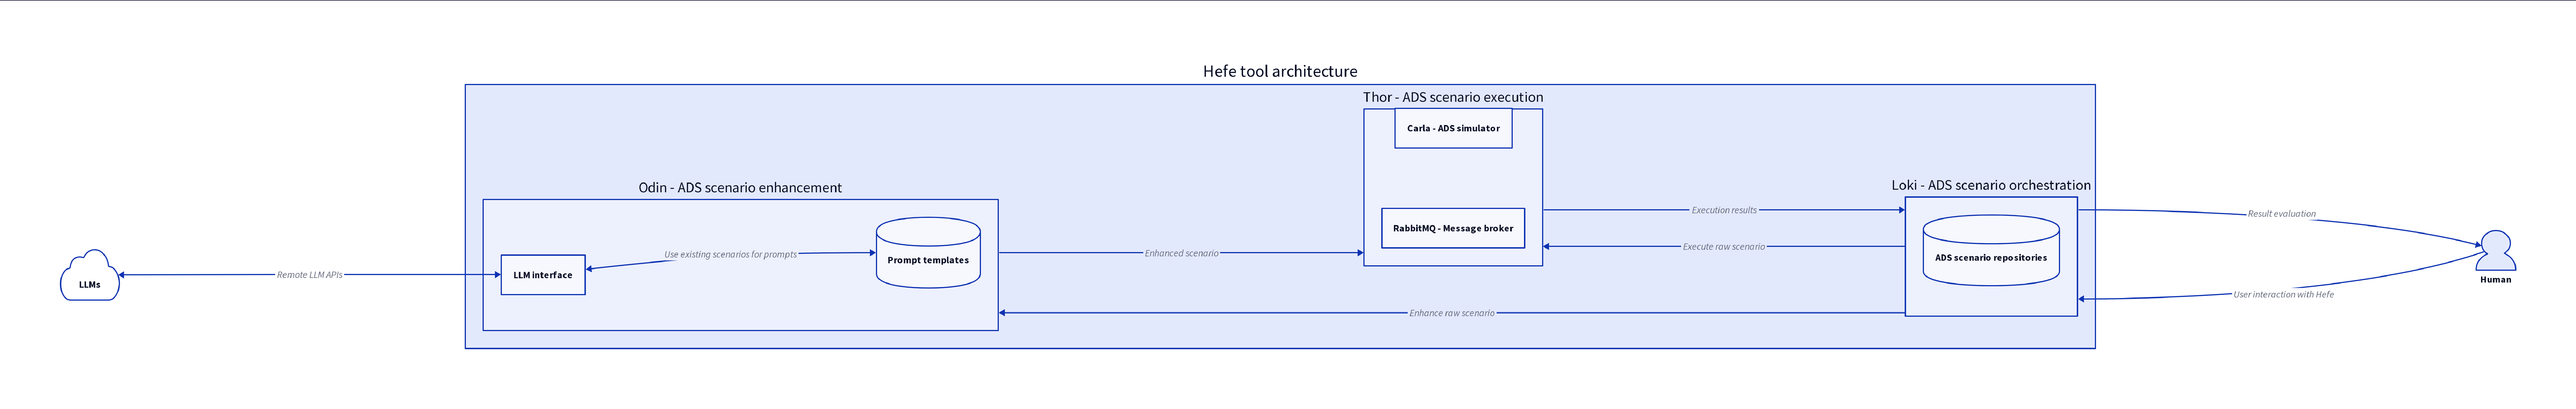
\includegraphics[width=\textwidth]{figures/d2-pdf/hefe.pdf}
    \caption{\hefe~pipeline architecture}\label{fig:hefeArch}
\end{figure}


Furthermore, as outlined in \citeauthor{LLM4AD}, \acrlongpl{llm} can be applied to several aspects
of \acrlong{ads}. It is not feasible that we focus on \textit{all} these aspects, and as such we
should narrow down our scope. Let us review some of the relevant aspects.

% Vi vil fokusere på driveability

% \section*{The applicability of \acrshortpl{llm} in \acrshort{ads} testing}
\section{Broad architectual overview}


\acrlong{ads} are typically modular, as we have seen in \Cref{sec:adsTestingComplexity}.
\acrshortpl{llm} are applicable to the different modules in different ways as we saw in
\Nref{sec:relatedWork}.
% TODO: Make more specific reference to what part of Related Work

\begin{tcolorbox}[colback=gray!5!white,colframe=gray!75!black,title=User history
        of using \hefe]\label{user-history}
    I have a set of \acrfull{ads} test cases. I provide this set to \hefe. It will run the entire
    set, and generate a baseline of my \acrshort{ads} performance.

    \hefe~will then improve my test cases using \acrlongpl{llm} and run them again.

    Lastly \hefe~will report how the results differ from running the base and enhanced version of a
    test case.

    This will give me insight into what caused my \acrshort{ads} to fail so that I can look into the
    cause of the error state and uncover underlying faults in the \acrlong{ads}.

\end{tcolorbox}


\subsection{Implementation language}

The programming language \textsc{Python} is widely used for \acrfull{ads} simulation. It is a high
level language, allowing the user great flexibility and developer experience. For this reason, I will
implement \hefe~using Python.

Python can be optimized using \acrfull{jit} compilers such as Numba~\cite{numba}, which can speed up
our execution times. Libraries such as Joblib provide Python with plug-and-play
meomization, which will allow us to re-use values that have already been
computed, saving time and energy.


\subsection{Overview of the components of the \hefe~pipeline}

The pipeline architecture is visualised in \Nref{fig:hefeArch}. Here we
present the major components and their responsibilities


\subsubsection{Test case enhancement}

\subsubsection{Test case repositories}

We have seen in \Nref{sec:relatedWork} that there are existing repositories of
% TODO: Make more specific reference to what part of Related Work
\acrshort{ads} test cases. These will provide us with \begin{inparaenum}
    \item a baseline,
    and
    \item data onto which we can apply our \acrshort{llm} enhancements.
\end{inparaenum}

\subsubsection{\acrshort{llm} enhancement}\label{sec:llmEnhancement}
% TODO: Dette må spisses mot driveability

The base test cases will individually be enhanced by prompting the
\acrshort{llm}. We will experiment with several \acrshortpl{llm}.

For performing the actual improvement, it is essential that we \begin{inparaenum}
    \item test several \acrshort{llm},
    \item give clear prompts
    % \info{I'm inclined to find some fitting prompts through trial and error, as such a I do not wish to describe them in detail at this time.}
    and
    \item verify that the returned test case adheres to the strictly necessary
    syntax rules. This last point is important due to our knowledge of
    \acrshortpl{llm} hallucinating (see \Nref{sec:llmProblems}).
    % TODO: More specific reference to Halucination intead of all LLm problems?
\end{inparaenum}

In order to facilitate testing various \acrlongpl{llm}, we should employ
\acrshort{llm} agnostic software as a translation layer. This will allow us to
write code for a common interface and test several \acrshortpl{llm} that may all
have different internal \acrfullpl{api} without having to modify our test code
for specific \acrshortpl{api}. This \begin{inparaenum}
    \item saves time
    and
    \item makes for more even test conditions \end{inparaenum}. Some pieces of software providing
this type of functionality include
\textsc{aisuite}\footnote{\url{https://github.com/andrewyng/aisuite}}, RamaLama from
RedHat\footnote{\url{https://github.com/containers/ramalama}}, and the MIT licensed
Ollama\footnote{\url{https://github.com/ollama/ollama}}, both supporting a plethora of
\acrlongpl{llm}.

\textsc{guidance}\footnote{\url{https://github.com/guidance-ai/guidance}} is a
framework for limiting the room in which \acrshortpl{llm} may operate, which
might be useful if we run into issues with excessive hallucination.


\subsubsection{Enhanced test case validation}

We must expect the \acrshort{llm} to hallucinate to some extent (\Cref{sec:llmHallucination}). We
therefore propose to verify the format of the enhanced file before running it.

As we saw in the section for \Nref{sec:adsScenarioFormats}, there exists several formats for
\acrshort{ads} scenarios. In order to verify that the syntax of our enhanced test
case is valid, we simply need to apply the syntax rules of our format.

The CommonRoad format is XML-based~\cite[720]{commonRoadOG} and as such we can
to some extent assess the degree of hallucination by parsing the XML structure.
Furthermore, it has an exhaustive Python library with several utilities\footnote{\url{https://pypi.org/user/commonroad/}}.

OpenSCENARIO exists both as XML and a domain-specific language (DSL). If we
utilise the XML version, we can apply the same methodology as for the CommonRoad
format. If using the DSL version, one way
the OpenSCENARIO format can be verified is by using free
online cloud services such as this offering from AVL
\footnote{\url{https://smc.app.avl.com/validation}}. We should however strive for
running a local verification service to \begin{inparaenum}
    \item save time and compute,
    and
    \item preserve data privacy.
\end{inparaenum}
Besides, it is generally a good idea to limit the number of external dependencies\footnote{Note for
    example how LGSVL\cite{lgsvl} was shut down, preventing projects such as DeepScenario of
    \citeauthor{DeepScenario} to be further developed on the original platform.}.

\subsection{Test case running and evaluation}

\subsubsection{Test case runner}

The system will automatically run all
our base test cases using an \acrshort{ads} simulator, and collect data points to get a baseline. It
will later also run the mutated \acrshort{llm}-enhanced versions of the base cases.

We have already ran the test cases in their base form. We will now run their
improved versions in order to compare them to see what effect the \acrshort{llm}
enhancement (see \Cref{sec:llmEnhancement}) has had.

For the reasons we have seen in~\Cref{sec:simulatorOverview}, we want to run our
test cases on Carla. It is the best offering as it is open source, under active
development and has a feature rich Python \acrshort{api}.

\subsubsection{Test case improvement evaluation}\label{sec:testCaseEval}

We saw in \Cref{sec:adsMetrics} that there are several metrics for assessing
\acrshort{ads}. We will use these metrics when evaluating our improvements.

\subsubsection{Test case result reporting}

We will compare the results from running
the baseline unmodified test case and comparing it with the results from
running the \acrshort{llm}-enhanced version and returning to the user. Ideally with
some automatic analysis of the results.

Having ran both the base test case and its enhanced counterpart, we have
results. The results will be stored in \acrfull{csv} files, allowing \begin{inparaenum}
    \item further analysis in Python/Jupyter,
    and
    \item easy translation to \LaTeX tables for the final report.
\end{inparaenum}

This is the final step of the envisioned pipeline. Where we have our result, and
need to analyse them.

This last step has great opportunities for being scoped up to a fully integrated
test suite which allows for both running test cases and analysing the results in
a \acrfull{gui}. But we should focus on the prior steps for now, only creating a
\acrshort{gui} if there is sufficient time towards the end of the project to
focus on such non-\acrshort{llm} related topics.

Initially, the results will consist of numerical comparison of the
\acrshort{csv}s with regard to the relevant metrics outlined in
\Nref{sec:testCaseEval}.

We need to define what requirement we will use for determining the \textit{result} of a test case
run. Without this, we cannot compare it to other test cases.

\section{Component details}

Having begotten a broad overview of the details of the \hefe pipeline, let us now narrow our scope
and focus on the individual components.

% Alt under her er kopiert over fra det gamle "implementation details"-chpt.
% (Og så tilpasset litt, dekrementert heading levels osv )


The implementation is what facilitates doing the actual experiments. For the
most part, it follows what is outlined in the \Nref{sec:solutionProposal}, with
some minor practical differences.
What follows will analyze the impelementation of the components of the \hefe{}
pipeline and explain more closely in detail not only \emph{what} they do, as
that is already covered in the solution proposal, but \emph{how} they do it, with
hands-on code examples.

% TODO: Burde avklare om den skal leve her "for alltid". Syns det kan gi emning
% å samle alle master ting i ett repo. Fortrinnsvis _dette_ (veldig meta å linke
% til seg selv i så fall hehe). Kan også være gunstig mtp å inkludere kode som appendix?
All code is available on the Github repo \href{https://github.com/orjahren/master-hefe}{\texttt{master-hefe}}.

\subsection{Carla interface and scenario utilities -- Thor}

The Thor module is responsible for all thigs related to the Carla \acrshort{ads}
simulator. It provides the client with several scenario-related utilities, and
is capable of executing the desired scenarios.


Certain of its utilities are simple tools for asserting the liveness of Carla,
such as the \texttt{get\_carla\_is\_up} function, shown in
listing~\ref{lst:odinCarlaHealthCheck}. This function will use the Caral
standard Python library and attempt to connect to the server on its default
port\footnote{I.e. \num{2000}, line \#4 in listing
    \ref{lst:odinCarlaHealthCheck}.}. Note that we refer to the host as simpyly
\texttt{carla} -- this is possible due to the entire project running
containerised with Docker Compose. Instead of refering to the speicifc IP
address of the Carla server (typically localhost, if not running it externally),
the Docker system will facilitate this name translation for us.

\begin{lstlisting}[caption={Exerpt from carla\_interface.py, demonstrating the implementation of a Carla health check.}, label={lst:odinCarlaHealthCheck}, language={Python}]
import carla

CARLA_HOST = "carla"
CARLA_PORT = 2000


def get_carla_is_up() -> bool:
    """
    Check if the CARLA simulator is up and running.
    This function attempts to connect to the CARLA server and returns True if successful, otherwise False.
    """
    print("Running carla integration check to see if it is up...")
    try:
        client = carla.Client(CARLA_HOST, CARLA_PORT)
        client.get_world()
        return True
    except Exception as e:
        print(f"CARLA connection failed: {e}")
        return False
\end{lstlisting}

This is used both to assert the general liveness of the \hefe pipeline, and to
verify that the simulator is available before performing experiments. It is
better to detect this illegal state \emph{before} running experiments rather
than during their execution.

Furthermore, it shall also be equipped with funcitonality for \emph{executing} \acrshort{ads}
scenarios on Carla. This is trivial when using Carla's existing Scenario Runner
module's funcitonality. As of now, this has not yet been implemented due to
greater challenges in the \acrshort{llm} module -- Odin.


% Rest API - running test cases - Thor
% “Fast API”, Python
% POST a test case to the API. It will be ran on the ‘server’
% RabbitMQ for listening for finished test cases? So that the client knows it can fetch the results?
% Will need UUID for test cases so the correct result can be fetched after it has been ran
% Need to store these somewhere. NoSQL database?
% This component should also accumulate results.
% Huge TODO: What metric are these results?
% Should be containerised (Docker/Podman)

\subsection{LLM interface and prompt applications -- Odin}\label{sec:odinImplementation}

% Rest API - performing LLM enhancement - Odin
% “Fast API”, Python
% Take a base test case as body
% Have some prompt repository
% Apply prompts with LLMs
% Must integrate with LLM. Either locally (Ollama) or remote (some API)
% Look into good LLM agnostic transition layer. E.g. Aisuite
% https://github.com/andrewyng/aisuite
% Should use same UUIDs as outlined above, but suffixed with e.g. “pure” and “tainted”
% Containerized. Docker compose?

The Odin module handles all things \acrshort{llm}. It provides a unified
\acrshort{api} for applying various prompts to scenarios and returning the
enhanced output resulting from having applied the prompt. We hve implemented
support for the \acrshortpl{llm} that are available on \begin{inparaenum}
    \item Ollama, and
    \item Gemini
\end{inparaenum}. This allows for testing with \acrshortpl{llm} such as
\begin{inparaenum}\setcounter{enumi}{2}
    \item Mistral \num{7.2}B, and
    \item gemini-2.5-flash
\end{inparaenum}.

\subsection*{LLM interface implementations}
\subsubsection{Gemini integration}

The Gemini integration is quite straightforward, relying on Google's own
\texttt{genai} Python module. Listing~\ref{lst:thorGeminiInterface} renders the
\emph{entire} interface, again highlighting how straightforward this really is.
The one piece of complexity to not is that it requires that the user provides
their own Gemini \acrshort{api} key and has this set as an environment variable
with the proper name. Without this being as it should, the script will crash, as
it would not possible for it to complete the desired \acrshort{llm} enhancement
regardless as long as the \acrshort{api} key is not present.

\begin{lstlisting}[caption={llm\_api\_interfaces/gemini\_interface.py, The implementation of a Gemini interface for executing prompts.}, label={lst:thorGeminiInterface}, language={Python}]
import os


from google import genai


def get_api_key() -> str:
    api_key = os.getenv("GEMINI_API_KEY")
    if not api_key:
        raise EnvironmentError("GEMINI_API_KEY environment variable not set.")
    return api_key


client = genai.Client(api_key=get_api_key())


def api_is_up():
    return True  # Assume Google never dies...


# TODO: Use decorator for asserting API liveness? Or standard assertion??
def execute_gemini_model(model_name: str, prompt: str) -> str:

    response = client.models.generate_content(
        model=model_name or "gemini-2.5-flash",
        contents=prompt
    )

    return response.text
\end{lstlisting}

\subsubsection{Ollama integration}

The Ollama integration is a bit more cumbersome. This motly comes down to it not
using any exisitng library modules for this specific purpose, instead relying on
using the \texttt{json} and \texttt{requests} modules to implement the desired
funcitonality from scratch, making it so that we need to handle network IO and
marshalling the \acrfull{llm} response into a fitting return buffer.

Listing~\ref{lst:thorOllamaInterface} renders the
\emph{entire} interface. As we can see, it is not too bad allthough nowhere near
as clean as the Gemini implementation (\ref{lst:thorGeminiInterface}).

Its complexity arises principally from \num{2} major factors --
\begin{inparaenum}
    \item the already mentioned manual networking, and
    \item having to parse the streamed response
\end{inparaenum}
Furthermore, this code expects that the user already \emph{has} an Ollama
installation running on their host machine. The code provides no means of setup
for this -- that is an entirely external endeavour that is left up to the end user.

Similarly to how the Gemini implementation does it, this will crash if Ollama is
not funcitoning properly as it would not possible for it to complete the desired
\acrshort{llm} enhancement regardless if Ollama is unreachable.

\begin{lstlisting}[caption={llm\_api\_interfaces/ollama.py, The implementation of an Ollama interface for executing prompts.}, label={lst:thorOllamaInterface}, language={Python}]
import json
import requests


OLLAMA_API_URL = "http://localhost:11434"


def api_is_up():
    try:
        response = requests.get(OLLAMA_API_URL)
        return response.status_code == 200
    except requests.ConnectionError:
        return False


# ollama models
def get_ollama_models():
    try:
        response = requests.get(f"{OLLAMA_API_URL}/api/tags")
        if response.status_code == 200:
            return response.json()["models"]
        else:
            print(f"Failed to get models: {response.status_code}")
            return []
    except requests.ConnectionError:
        print("Failed to connect to the API.")
        return []


# TODO: Use decorator for asserting API liveness? Or standard assertion??
def execute_ollama_model(model_name: str, prompt: str):
    try:
        payload = {
            "model": model_name,
            "prompt": prompt
        }
        print(f"Executing model {model_name} with prompt: {prompt}")
        response = requests.post(
            f"{OLLAMA_API_URL}/api/generate", json=payload)
        if response.status_code == 200:
            result = ""
            for line in response.iter_lines():
                if line:
                    data = line.decode('utf-8')
                    try:
                        json_obj = json.loads(data)
                        result += json_obj.get("response", "")
                    except Exception as e:
                        print(f"Failed to parse line: {e}")
            return {"text": result}
        else:
            print(f"Failed to execute model: {response.status_code}")
            return None
    except requests.ConnectionError:
        print("Failed to connect to the API.")
        return None
\end{lstlisting}

\subsection*{Prompts and their associated code}

In this project, the prompts are the instruction to the \acrfull{llm} for
applying the enhancement to the scenario. Quite possibly the most critical piece
of code related to the experiments. They need to take the base scenario as an
input and integrate it into the \acrshort{llm} context, such that it knows what
it shall use as its base to apply enhancements that will decrease the
driveability. For this reason, it also provides certain scenario
utilities\footnote{That architectually might as well have been integrated in the
    Thor module\ldots}.

\subsubsection{Scenario utilities}

These are essentially quite trivial helpers. Lisitng \ref{lst:odinScenarioUtils}
render the core functionality -- hopefully this is quite self-explaining.

\begin{lstlisting}[caption={scenario\_utils.py, The implementation of an various scenaro helper functions for executing prompts.}, label={lst:odinScenarioUtils}, language={Python}]
import os


# TODO: Implementer denne
# TODO: Fastslaa hvilket format vi bruker (OpenSCENARIO/CommonRoad/andre)
def file_format_is_valid(file_format: str) -> bool:
    """
    Check if the file format is valid.

    Args:
        file_format (str): The file format to check.

    Returns:
        bool: True if the file format is valid, False otherwise.
    """
    return file_format in ["json", "yaml", "yml", "csv", "txt"]


def enumerate_enhanced_scenarios(scenario_repository_path: str, scenario_name: str) -> int:
    """
    Enumerate enhanced scenarios in a given scenario path.

    Args:
        scenario_repository_path (str): The path to the scenario directory.
        scenario_name (str): The name of the scenario.

    Returns:
        int: The number of enhanced scenarios found.
    """
    # TODO: Can probably refactor this
    acc = 0
    for scenario in os.listdir(scenario_repository_path):
        print(f"Checking scenario: {scenario}")
        if scenario_name in scenario and "enhanced" in scenario:
            acc += 1
    return acc


# TODO: Should use better names. Need a way of tracking enhanced scenario
# metadata
# - Timestamp
# - What prompt was used
# - What model was used
# - What the original scenario was
# - What changes were made?
def get_enhanced_scenario_name(scenario_repository_path: str, scenario_name: str) -> str:
    """
    Get the enhanced scenario name.

    Args:
        scenario_repository_path (str): The path to the scenario directory.
        scenario_name (str): The base name of the scenario.

    Returns:
        str: The enhanced scenario name.
    """
    num_enhanced_scenarios = enumerate_enhanced_scenarios(
        scenario_repository_path, scenario_name)
    if num_enhanced_scenarios == 0:
        return f"{scenario_name}-enhanced"
    else:
        # Big brain time...who needs UUIDs when you can just count files?
        return f"{scenario_name}-enhanced-{num_enhanced_scenarios + 1}"


def get_available_scenarios(scenario_repository_path: str) -> list:
    def extension_is_ok(filename: str) -> bool:
        # TODO: Verify which formats we want to support
        return filename in ["xosc", "py"]

    return [filename for filename in os.listdir(scenario_repository_path) if extension_is_ok(filename)]


# TODO: Should strip newlines??
def scenario_path_to_string(scenario_path: str) -> str:
    with open(scenario_path, 'r') as file:
        return file.read()


# TODO: Let this function determine output file name?
def save_enhanced_scenario(scenario_str: str, output_path: str):
    with open(output_path, 'w') as file:
        file.write(scenario_str)
\end{lstlisting}

\subsubsection{Prompts -- templating and usage}

% TODO: Finnes det noe bigbrain måte å slippe å manuelt måtte referere ti llinjenummer?
As mentioned, the prompts need to include the scenarios \emph{in} them, so that
they are accessible to the \acrshort{llm}. How this is done, is rendered in
listing~\ref{lst:odinPromptTestbed}. The most interesting aspect is how the
prompts are stored in the system as lambda functions. This makes it so that they
can take an argument that represents the scenario --
\texttt{python\_carla\_scenario\_raw}(line \#16) -- and simply \emph{execute} the
function to insert the scenario into the prompt (line \#42). This is then
inserted into the output prompt at the location located at line \#21 in the listing.

\begin{lstlisting}[caption={experiments/testbed/prompts.py, The implementation of a prompt testbed for executing prompts.}, label={lst:odinPromptTestbed}, language={Python}]
# We wish to decrease the driveability of the scenario by enhancing it with more
# details, increasing its complexity

# Prompt structure:
"""
1 - Context: We are working with a driving simulation environment for the Carla simulator.
2 - Task: Decrease the driveability of the scenario by enhancing it with more details and complexity.
3 - Input: <scenario_description, in python carla scenario format>
4 - Output: An enhanced version of the scenario description with additional
details and complexity, still in Python carla scenario format. ONLY output the
code, without any additional text or explanation.
"""

PROMPTS = [
    [...] # NOTE: Removed most prompts from this listing for brevity.
    lambda python_carla_scenario_raw: f"""
    1 - Context: You are a tool for decreasing the driveability of scenarios in the driving simulator Carla.
    2 - Task: Decrease the driveability of the scenario by enhancing it with
    more details and complexity, using only methods that are part of the
    official Carla API, version 0.9.15.
    3 - Input, the Python specification for the scenario: {python_carla_scenario_raw}
    4 - Reasoning: Think step by step about how to make the scenario more complex and less driveable, considering possible obstacles, traffic, weather, and other factors using only the official Carla API.
    5 - Output: Only output the enhanced scenario code in Python Carla scenario format, with no additional text or explanation.
    """,
]


def name_to_prompt_idx(name: str) -> int:
    mapping = {
        "basic": 0,
        "no_explanation": 1,
        "no_explanation_strict": 2,
        "cot": 3,
        "cot_strict_methods_in_file": 4,
        "cot_strict_carla_api": 5,
    }
    return mapping.get(name, 0)


def get_prompt_for_python_scenario_enhancement(python_carla_scenario_raw: str, prompt_name: str) -> str:
    prompt_idx = name_to_prompt_idx(prompt_name)
    return PROMPTS[prompt_idx](python_carla_scenario_raw)

\end{lstlisting}

Lastly, note the comments in the top of the file, intended to give Github
Copilot increased understanding of the context, so that it can provide better
aid during programming.


\subsection{Execution tool / user oriented frontend -- Loki}

% Client - orchestrating the process - Loki
% Fetch available test cases from Thor? Select what/which are to be used
% Store results clientside? Separate database for this?

The final module of the \hefe pipeline is Loki -- it is simply a tool intended
to be used by the user for operating the process. It \begin{inparaenum}
    \item  says what scenarios are available to it (i.e. those that are eligble for
    being enhanced), and
    \item allows the user to select a prompt and
    \item execute that prompt to the scenario of their choosing.
\end{inparaenum}


\begin{lstlisting}[caption={loki/main.py, The implementation of the Loki script.}, label={lst:lokiMainImplementation}, language={Python}]
import pika
import requests

# from odin.server import ODIN_PORT
# from thor.server import THOR_PORT

ODIN_PORT = 4000
THOR_PORT = 6000


# TODO: Merge health checks into a single function?
def do_thor_health_check():
    try:
        res = requests.get(f"http://localhost:{THOR_PORT}/health")
    except requests.ConnectionError:
        print("Thor server is not running or unreachable.")
        exit(1)
    if res.status_code == 200:
        # parse json
        health_status = res.json().get("status", "unknown")
        if health_status == "healthy":
            print("Thor is healthy.")
        else:
            print(f"Thor health check failed.: {health_status}")
            exit(1)
    else:
        print("Thor health check failed.")
        exit(1)


def do_odin_health_check():
    try:
        res = requests.get(f"http://localhost:{ODIN_PORT}/health")
    except requests.ConnectionError:
        print("Odin server is not running or unreachable.")
        exit(1)
    if res.status_code == 200:
        health_status = res.json().get("status", "unknown")
        if health_status == "healthy":
            print("Odin is healthy.")
        else:
            print(f"Odin health check failed.: {health_status}")
            exit(1)
    else:
        print("Odin health check failed.")
        exit(1)


def run_test_case(test_case_id):
    print(f"Running test case: {test_case_id}")

    # Run test case on Loki
    result = requests.post(
        f"http://localhost:{THOR_PORT}/run_test_case",
        json={"test_case_id": test_case_id})
    if result.status_code != 200:
        print(f"Failed to run test case: {test_case_id}")
        return None
    print(f"Test case {test_case_id} executed successfully.")
    value = result.json().get("result", "No result found")
    return value


def get_enhanced_test_case(test_case_id):
    print(f"Enhancing test case: {test_case_id}")

    # Enhance test case on Odin
    result = requests.post(
        f"http://localhost:{ODIN_PORT}/enhance_test_case",
        json={"test_case_id": test_case_id})
    if result.status_code != 200:
        print(f"Failed to enhance test case: {test_case_id}")
        return None
    print(f"Test case {test_case_id} enhanced successfully.")
    value = result.json().get("result", "No result found")
    return value


def get_improvement(base_test_case, enhanced_test_case):
    # Simulate getting an improvement between two test cases
    # TODO: Implement actual logic to compare test cases
    return f"Improvement from {base_test_case} to {enhanced_test_case}"


def send_test_message(message):
    # TODO: Implement proper credentail handling.
    credentials = pika.PlainCredentials('user', 'pass')
    connection = pika.BlockingConnection(
        pika.ConnectionParameters('localhost', credentials=credentials))
    channel = connection.channel()
    channel.queue_declare(queue='test_queue')
    channel.basic_publish(exchange='', routing_key='test_queue', body=message)
    print(f"Sent message to RabbitMQ: {message}")
    connection.close()


if __name__ == "__main__":
    print("Loki is running...")

    do_thor_health_check()
    do_odin_health_check()

    send_test_message("Hello from Loki!")

    exit(0)
    test_case_id = "test_case_123"

    print("Starting test case execution...")
    base_result = run_test_case(test_case_id)
    print(f"Base result: {base_result}")

    enhanced_test_case = get_enhanced_test_case(test_case_id)

    enhanced_test_case_result = run_test_case(enhanced_test_case)
    print(
        f"Enhanced test case execution completed with result: {enhanced_test_case_result}")

    improvement = get_improvement(base_result, enhanced_test_case_result)
    print(f"Improvement: {improvement}")

    print("Loki execution finished.")

\end{lstlisting}


Listing~\ref{lst:lokiMainImplementation} renders the implementation of the
script. It relies on the Odin and Thor modules for all essential functionality,
which is in line with what is to be expected as this is simply a frontend client
to \emph{reach} them.

It is relies on the \texttt{requests} module for doing \acrfull{rpc} to the
other modules. There is also the outlines of a RabbitMQ implementation, which is
why \texttt{pika} is being imported. As of now, this is in non-functioning
alpha. Implementation of RabbitMQ message passing has not been prioritized as
there were, as mentioned, more important issues to focus on that would yield
better and more important results when resolved. This would maintain feature
parity with the \texttt{requests}-based approach.
% \newpage
% \section{Potential Future Work}

\subsection{Temperature}
Hallucination.

\subsection{More models}
More models more good?

\subsection{Instant validation of test case syntax}
Compiler-stuff. Syntax. Parsing.

\subsection{Relevant pretraining?}

\subsection{Retrieval-augmented generation (RAG)}
Context, affordances.

\printbibliography[]

\end{document}


 \usepackage{glossaries}
 \setglossarystyle{altlist}

\newcommand{\hefe}{\textsc{Hefe}}

\setdefaultenum{(1)}{(a)}{i.}{A.}
\interfootnotelinepenalty=10000 

\addbibresource{refs.bib}

\newacronym{llm}{LLM}{Large Language Model}
\newacronym{llms}{LLMs}{Large Language Models}
\newacronym{ads}{ADSs}{Autonomous driving systems} 
\newacronym{ad}{ADS}{Autonomous driving system} 
\newacronym{jit}{JIT}{Just-In-Time} 
\newacronym{ml}{ML}{Machine learning} 
\newacronym{dl}{DL}{Deep learning} 
\newacronym{api}{API}{Application programming interface} 
\newacronym{apis}{APIs}{Application programming interfaces} 
\newacronym{csv}{CSV}{Comma separated values} 
\newacronym{gui}{GUI}{Graphical user interface} 
\newacronym{cv}{CV}{Computer Vision} 
\newacronym{dsc}{DSC}{Driving situation complexity}
\newacronym{icl}{ICL}{In-context learning}
\newacronym{cot}{CoT}{Chain-of-Thought}
\newacronym{rl}{RL}{Reinforcement learning}

\begin{document}

\frontmatter
\pdfbookmark{Title Page}{titlepage} % add PDF outline entry
\thispagestyle{empty} % no number on the title page
\begin{center}
    \begin{adjustbox}{center}%,trim=0 0.2cm 4cm 0.2cm}
        % \includegraphics[width=1.4\textwidth]{MFF-logo.pdf}
        
\includegraphics[width=0.4\textwidth]{uio-seal.eps}
    \end{adjustbox}

    \Large

    \vspace{-2em}
    \vfill

    {\ifFANCY\sffamily\Huge\else\bfseries\LARGE\fi
        \MakeUppercase{\ThesisType} ESSAY}

    \vfill

    {\Huge
        \ThesisAuthor}

    \vspace{1em}

    %% if `\ThesisTitleFront` is not defined, use `\ThesisTitle`
    \ProvideExpandableDocumentCommand{\ThesisTitleFront}{}{\ThesisTitle}
    % {\Huge \bfseries \ThesisTitleFront \par}
    {\fontsize{30pt}{36pt}\selectfont \bfseries
        \ThesisTitleFront \par}

    \vfill

    \Department

    \vspace{1.1em}

    \begin{center}
        \small
        \renewcommand{\arraystretch}{1.2}
        \begin{tabular}{>{\sffamily\color{Gray40}}r @{\hspace{1.0em}} l}
            Supervisor of the Thesis    & \Supervisor     \\
            \ifdef{\CoSupervisor}{%
            Co-Supervisor of the Thesis & \CoSupervisor   \\
            }{}
            \ifdef{\StudyProgramme}{% TODO: programme vs program?
            Study Programme             & \StudyProgramme \\
            }{}
        \end{tabular}
    \end{center}

    \vspace{2em}

    \ifFANCY\sffamily\fi
    Oslo \YearSubmitted \\
    \ifdef{\YearRevision}{%
        \emph{Revised version \YearRevision} \par
    }{}
    \ifWIP
        \small\ttfamily \textcolor{red}{(Draft - \today)} \par
    \fi
\end{center}

\newpage

\contentsandlists

\mainmatter
\chapter{Introduction}

% \epigraph{The whole is greater than the sum of its parts.}{Aristotle}

\section{Motivation}

\textbf{Conventional cars} are ubiquitous in society. Whether for freight trafficking or for humans, cars have great flexibility with their ability to go wherever without requiring tailored infrastructure
such as railway tracks. They do, however, have one major weak point --- the human driver. For this
reason, industry and academia have put forward efforts to enhancing cars with \acrfull{ads}
capabilities.
By \textbf{empowering humans} with autonomous vehicles, it is expected that traffic efficiency will
increase and road fatalities will fall.

\textbf{Due to the critical safety situation of manoeuvring a car} In a public setting where other external
actors are present, it is essential that \acrlongpl{ads} are thoroughly tested before they are
deployed so that they are confirmed to be sufficiently safe and capable of handling the situations in which
they may typically end up.
But due to the complicated nature of the typical \acrshort{ads} operating environment, coming up with
exhaustive system test solutions is near impossible.
For this reason we want a way of testing the system that is capable of pushing the \acrlong{ads} to
its limits such that we can measure its performance and see if it is capable of
handling complex scenarios.

\textbf{Having an existing repository of \acrlong{ads} test cases,} such as
DeepScenario we wish to improve them. \textbf{\acrfullpl{llm}} have demonstrated
great capabilities of context learning and emergent abilities, which begs
the question of their  applicability for \acrshort{ads} testing.  There are
various methods of testing  \acrlong{ads}. Can these existing test methods be
improved by applying \acrshort{llm} technology to them?

% Yet, testing is \textit{important} for \acrlong{ads}, and text case generation is costly. We
% therefore pose the question: Can \acrshort{llms} be applied for (1) lowering the
% cost of testing, and (2) increasing the thouroughness of \acrlong{ads} testing?

\newpage % Legger inn en ny side siden thesis overview uansett konsumerer den siden

\section{Research questions}

TODO: formalize research questions.

\section{Thesis overview}

The thesis is structured as follows:

\begin{itemize}
    \item \Cref{sec:background} introduces key concepts related to \acrshortpl{ads} and \acrshortpl{llm}.
    \item \Cref{sec:problemDescription} defines the specific problem addressed in this work.
    \item \Cref{sec:literatureReview} reviews the current state of research in the field.
    \item \Cref{sec:relatedWork} discusses related applied works and lessons learned.
    \item \Cref{sec:solutionProposal} details our proposed solution and its technical aspects.
    \item \Cref{sec:experiments} describes the experimental setup used to evaluate the solution.
    \item \Cref{sec:results} presents the findings from the experiments.
    \item \Cref{sec:discussion} analyzes and compares the results to existing work.
    \item \Cref{sec:furtherWork} suggests directions for future research.
    \item \Cref{sec:conclusion} summarizes the main contributions and findings.
\end{itemize}

Two appendices are included: \Nref{sec:fileDiffs} and \Nref{sec:errorMessages}.

\chapter{Background}

\epigraph{The limits of my language mean the limits of my world}{Wittgenstein}

\section{Testing}

First, we need to establish some basic testing concepts.

\subsection{Pre- and post-conditions}\label{sec:testingConditions}

When running test cases, the concept of \textit{Pre-conditions}
refers to certain properties that
obtain \textit{before} running a given test case. E.g that the \acrshort{ads} ego vehicle is
stationary.

In many ways mirroring pre-conditions, \textit{post-conditions} refers to the properties that obtain
\textit{after} having ran a test. E.g. that the ego vehicle will be moving after having performed
the test.

% TODO: The testing conditons should ideally be cited.

\subsection{Test coverage}\label{sec:testCoverage}

\textbf{Test coverage} refers to the what degree the entire system is being tested. The concept can
be used to describe both hardware and software test
coverage~\cite[187]{testCoverage94}.~\citeauthor{testCoverage94} posit that hardware-based test
coverage is measured in terms of the number of possible faults covered, whereas software-based test
coverage is measured in terms of the amount of structural or data-flow units that have been
exercised~\cite[187]{testCoverage94}. A test case that exercised every single code line of the
system would by definition have perfect test coverage.


% \subsection{Autonomous systems}
% 
% Autonomous systems are systems that are capable of changing their behaviour in
% response to unanticipated events during
% operation~\cite[368]{watson2005autonomous}. Autonomous systems exist in several
% different forms and they are typically tailored for their specific operating
% environments. Some systems operate in the maritime domain, some in the air, and
% others on the ground in the terrestrial operating domain~\cite[369-370]{watson2005autonomous}.

\section{\acrfullpl{ads}}

\acrfull{ads} are systems that enable automotive vehicles to drive autonomously. Due to the typical
operating scenarios of a car it is pivotal that the \acrlong{ads} maintain a high safety standard. A
common way to assert safety is to use simulator based testing~\cite[1]{DeepScenario}.

\subsection{\acrlong{ads} testing}

Testing is essential for assuring \acrlong{ads} operative safety~\cite[163]{ADTestingReview16}.
Several methods for testing exist, testing various aspects of the \acrlong{ads}. An \acrshort{ads}
typically exists of several modules, all working together and handling different aspect of the
\acrlong{ads}.

\citeauthor{ADTestingReview16} outline several typical architectures for \acrshort{ads} testing,
drawing on traditional software testing traditions outlining how \textit{software testing} can be
used alongside more specialized \acrshort{ads} testing techniques such as \textit{simulation
    testing} and \textit{X-in-the-loop testing}~\cite[163-164]{ADTestingReview16}.

\subsection{\acrlong{ads} driveability}\label{sec:adsDrivability}

\textbf{Driveability} is a high-level estimator of the overall driving
condition of an \acrshort{ads}, derived from several lower-level sources~\cite[3140]{safeToDrive}.
It can be used to refer to various aspects of a scene.
\citeauthor{safeToDrive} discuss the concept further, using the  scene definition
of~\citeauthor{scenes} as outlined in  \Cref{sec:adsSimConcepts}, they describe
how driveability can refer both to \begin{inparaenum}
    \item road conditions, and
    \item human driver performance.
\end{inparaenum}
\citeauthor{safeToDrive} go on to give an overview of how driveability
can be used to refer to a \begin{inparaenum}\setcounter{enumi}{2}
    \item \textit{driveability map} which divides a map into
    cells indicating where the \acrshort{ads} expects that it will be able to go, and
    \item \textit{object driveability}, which refers to the classification of physical objects in
    the environment that the \acrshort{ads} expects that it can run over without causing damage to
    the ego vehicle~\cite[3135-3136]{safeToDrive}.
\end{inparaenum}

The main method for assessing the driveability of a scene comes form assessing the environment of
the scene. Factors such as \begin{inparaenum}
    \item weather,
    \item traffic flow,
    \item road condition, and
    \item obstacles \end{inparaenum} all play into this. The \acrshort{ads} infers information from
observation~\cite[3136]{safeToDrive}.

They continue to give an overview of various \textit{driveability factors} and their associated
difficulties, using a a split between \textit{explicit} and \textit{implicit} factors.

\textbf{Explicit driveability factors} will typically include factors such as \textbf{Extreme
    weather} such as \begin{inparaenum}
    \item fog,
    \item heavy rain,
    \item snow,
\end{inparaenum}
all serving to impair road visibility and causing increased difficulties for vision-based tasks such
as road detection and object tracking~\cite[3136-3137]{safeToDrive}. \textbf{Illumination} also
poses various challenges for typical \acrshort{ads} tasks as a typical \acrshort{ads} will be
required to operate in a plethora of scenes with varying degrees of illumination depending on
factors such as time of day and location (e.g. if the \acrshort{ads} is operation in a dimly lit
tunnel)~\cite[3137]{safeToDrive}. The authors highlight how low illumination may serve as an
advantage for the \acrshort{ads} as this allows for using the head lights of other vehicles as a
feature for detecting them, whereas it make pedestrian detection significantly more
challenging~\cite[3137]{safeToDrive}. \textbf{Road geometry} is another external factor, satisfying
our natural intuition that \textit{intersections} and \textit{roundabouts} are more difficult to
drive through than straight highways~\cite[3137]{safeToDrive}.

\textbf{Implicit driveability factors} consist of behaviours and intent of other road users
interacting with the autonomous car~\cite[3138]{safeToDrive}. This includes the actions of other
vehicles such as their \begin{inparaenum}
    \item overtaking,
    \item lane changing,
    \item rear-ending,
    \item speeding, and
    \item failure to obey traffic laws \end{inparaenum}.~\citeauthor{safeToDrive} call these factors
\textbf{vehicle behaviours}~\cite[3138]{safeToDrive}. Furthermore, \textbf{pedestrian behaviours}
are also taken into account, noting how pedestrians can sometimes
\begin{inparaenum}\setcounter{enumi}{5}
    \item cross the road,
    \item be inattentive, or
    \item fail to comply with the traffic law \end{inparaenum}\cite[3138]{safeToDrive}. They go on
to describe the \textbf{driver behaviour} of other drivers pointing out how
\begin{inparaenum}\setcounter{enumi}{8}
    \item distraction, and
    \item drowsiness \end{inparaenum} can be factors that cause accidents even for
\acrshort{ads}-enhanced vehicles due to the other, manual, cars
interfering with their operation~\cite[3138-3139]{safeToDrive}. Lastly
\textbf{motorcyclist/bicyclist behaviours} cause their own source of implicit driveability factors:
The models and methods developed for analysing the group's behaviour are far more limited than other
groups of road users~\cite[3139]{safeToDrive}.~\citeauthor{safeToDrive} theorise that this comes
down to the lack of available datasets that capture and label the trajectories and behaviours
of motorcyclists and bicyclists~\cite[3139]{safeToDrive}, causing potential issues for any
\acrshort{ads} that wishes to operate in a shared traffic environment with this group.

\subsection{\acrlong{ads} testing metrics}\label{sec:adsMetrics}

When evaluating \acrshort{ads} testing, several metrics can be used. What metric to use will depend
on what the relevant test is measuring.

Building on what we have learnt about driveability (\Cref{sec:adsDrivability}),
we take after \citeauthor{safeToDrive} and review three metrics for
quantifying driveability: \begin{inparaenum}
    \item scene driveability,
    \item collision-based risk, and
    \item behaviour-based risk.
\end{inparaenum}

\textbf{Scene driveability} refers to how easy a scene is for an
\acrshort{ads} to navigate, and the \textit{scene driveability score} refers to
how likely the \acrlong{ads} is to fail at traversing the
scene~\cite[3140]{safeToDrive}. It is typically found through and end-to-end
approach. Note how this is a metric for \textit{scenes}, without taking into
account the performance of any specific \acrshort{ads}.

\textbf{Collision-based risk} comes in two kinds - \begin{inparaenum}
    \item binary risk indicator, and
    \item probabilistic risk indicator.
\end{inparaenum} \citeauthor{safeToDrive} posit that the prior, binary metric, indicates whether a
collision will happen in the near future in a binary `either-or' sense, whereas the latter yields a
probability calculated based on current states, event, choice of hypothesis, future states and
damage~\cite[3140]{safeToDrive}.

\textbf{Behaviour-based risk} estimation also represents a binary classification problem wherein
nominal behaviours are learnt from data, and then dangerous behaviours are detected on that. This
requires a definition of `nominal behaviour', which is typically defined on on acceptable speeds,
traffic roles, location semantics, weather conditions and/or the level of fatigue of the
driver~\cite[3140]{safeToDrive}. Furthermore \citeauthor{safeToDrive} describe how this metric also
allows more than one \acrshort{ads} to be labelled as `conflicting' or `not
conflicting'~\cite[3140]{safeToDrive}, representing a ruling on their compatibility. Finally, they
note how behaviour-based risk assessment typically focuses on driver behaviours, not taking into
account other actors in the scene such as pedestrians or cyclists.

\subsection{The complexities of \acrshort{ads} testing}\label{sec:adsTestingComplexity}

As we have seen, \acrshortpl{ads} can perform several tasks, in several environments. As such, there
are several relevant factors for testing them. It is not feasible to test all potential variations
of all potential environments in the real world, meaning that the \textit{test
    coverage}\footnote{See \Nref{sec:testCoverage}} typically will be low.

Some of the factors that complicate \acrshort{ads} operations are \begin{inparaenum}
    \item timing,
    \item sequence of events, and
    \item parameter settings such as the different speeds of various vehicles and other actors.
\end{inparaenum}

\citeauthor{adsComplexityIndex18} posit that \textit{the concept of complexity exists everywhere,
    but there is no agreement on one for driving situations}~\cite[1182]{adsComplexityIndex18}.
Therefore they introduce their own concept of \acrfull{dsc}, which serves to give a metric of a
the complexity of a given driving situation. Their \acrshort{dsc} is defined as the output of a
mathematical formula taking into account the perplexity and standard deviation of several
control variables $\mathcal{M}$ representing the surrounding vehicle's
behaviour~\cite[1182]{adsComplexityIndex18}. Their formula also takes into account the ratio of
\textit{V2X}-capable vehicles~\cite[1182]{adsComplexityIndex18}, i.e. the vehicles that are
connected and capable of communicating~\cite[1]{v2xTestingSurvey2019}.

% It is common to modularize the testing of \acrshort{ads} so that the individual modules can be
% tested in isolation. The modules of an \acrshort{ads} typically include a motion planner, a
% \acrfull{cv} system, and % LIDAR. This allows for testing the individual modules in a way that
% makes sense for their specific domains.

\subsection{\acrlong{ads} simulation}

Due to the complexity involved in testing \acrlongpl{ads} (\Cref{sec:adsTestingComplexity}),
simulators are typically used for this purpose~\cite{DeepScenario}. While the same points about not
being able to test \textit{all} possible scenarios do remain true for simulator based testing due to
the sheer number of factors, using a simulator allows for far greater testing at far lower cost due
to the minimal overhead of
\begin{inparaenum}
    \item generating,
    \item running, and
    \item evaluating the outcome of
\end{inparaenum}
test cases.

Furthermore, simulators allow for greater flexibility in determining the test scenarios due to not
being confined by the  physical world that is available to the scientist that wishes to perform the
testing. Using a simulator, a Europe-based scientist can test their \acrshort{ads} for North
American conditions, or vice-versa.

\subsection{The \acrshort{ads} simulator jungle}\label{sec:simulatorOverview}

Due to the appeal of running \acrshort{ads} simulation, several contenders exist
on the market.

\textbf{Carla} is a widely used \acrshort{ads} simulator~\cite{Carla}. It is implemented
using the game engine UnrealEngine~\cite{unrealengine} and allows for running
test cases under various scenarios and collecting their results. Carla is fully
open source and is under active development. It has been applied in projects such as KITTI-Carla,
which generated a KITTI dataset using Carla~\cite{kittiCarla}.

\textbf{LGSVL} is a deprecated simulator from LG~\cite{lgsvl}. It was used in projects such
as DeepScenario~\cite{DeepScenario}. It allowed for running various maps with various vehicles and
tracking their data. It was also capable of generating HD
maps \footnote{\url{https://github.com/lgsvl/simulator?tab=readme-ov-file\#introduction}}.
DeepScenario is a project similar to this, concerned with testing \acrlongpl{ads}. Further details
about it in are located in \Nref{sec:relatedWork}.

\textbf{AirSim} is Microsoft's offering~\cite{airsim}. It has, like LGSVL,
been deprecated. It is also built using UnrealEngine. Unlike the other
simulators we have seen, this also focused on autonomous vehicles outside of
only cars, such as drones.


\subsection{Concepts of \acrshort{ads} simulation}\label{sec:adsSimConcepts}

\citeauthor{scenes} draw up an outline for the terms \textit{scene}, \textit{situation}, and
\textit{scenario}, that are all concepts widely used in \acrshort{ads} simulation testing.

\textbf{scene} is a term that is used in different manners in various
articles~\cite[982]{scenes}, but \citeauthor{scenes} propose standardising the definition on
\textit{a scene describing a snapshot of the environment including the scenery and dynamic elements,
    as well as  as all actors’ and observers’ self-representations, and the relationships among those entities}~\cite[983]{scenes}.

\textbf{situation} is, like \textit{scene}, employed in various fashions. \citeauthor{scenes}
give a background detailing its usage ranging from \textit{"the entirety of circumstances,
    which are to be considered by a robot for its selection of an appropriate behaviour pattern in a
    particular moment'}\footnote{The translation from German is borrowed from \citeauthor{scenes},
    \cite[984]{scenes}}, in  \citeauthor{scenarioTysk}~\cite[3]{scenarioTysk} to
\citeauthor{schmidtScenario} introducing a distinction between \textit{the true world} in a formal
sense, and that being the ground truth upon which a situation is
described~\cite[892]{schmidtScenario}.

\citeauthor{scenes} propose to standardise on the definition of a situation being \textit{
    the entirety of circumstances, which  are to be considered for the selection of an
    appropriate behaviour pattern at a particular point of time}~\cite[985]{scenes}.

\textbf{scenario} refers to \textit{'the temporal development between several scenes in a sequence
    of scenes'}\cite[986]{scenes}. We note how the definition a a scenario utilises that of a scene.
Furthermore, \citeauthor{scenes} hold it to be the case that \textit{'every scenario starts with an
    initial scene. Actions \& events as well as goals \& values may be  specified to characterize
    this temporal development in a scenario'}~\cite[986]{scenes}, clarifying the distinction
between a scenario and a scene.

Lastly they posit that a scenario spans a certain amount of time, whereas a scene has no such
temporal aspect to it.


When running a simulation, we refer to the autonomous vehicle that is being
simulated as the \textit{ego vehicle}~\cite{egoDefinition}.

% introduce the concept of a \textit{scene}, which denotes 

% An alternate simulator is LG SVL~\cite{lgsvl}, but it has been deprecated since
% 2022 and as such it does not seem proper to build a new solution on top of it.
% The DeepScenario dataset~\cite{DeepScenario} utilises this simulator framework.
% \tanke{The LGSVL part can be removed - not relevant?}

\subsubsection{\acrshort{ads} scenario formats}\label{sec:adsScenarioFormats}

\textbf{OpenSCENARIO} is a standard developed by the Association for Automation and
Measurement Systems (ASAM), which is dedicated to the description of dynamic
scenarios~\cite[651]{generatingOpenScenario}. Under this format, only the
\textit{dynamic} content of the scenario is recorded in the file. The static
content is kept in other formats such as OpenDRIVER and
OpenCRG~\cite[652]{generatingOpenScenario}. The simulator Carla (outlined in
\Cref{sec:simulatorOverview}) supports this
standard~\cite[652]{generatingOpenScenario}.

Another widely popular scenario format is
\textbf{CommonRoad}~\cite[4941]{convOpenScenarioToCR}, first proposed in
\citedate{commonRoadOG}~\cite{commonRoadOG}. There are tools such as those
proposed by \citeauthor{convOpenScenarioToCR} that allows for converting
OpenSCENARIO scenarios to the CommonRoad
format~\cite[4941]{convOpenScenarioToCR}.

% TODO: Skrive om Carlas støtte for Python-scenarioer
% TODO: Skrive om Carla scenario runner her?

\section{\acrfullpl{llm}}

\acrfullpl{llm} are transformer-based language models that typically contain several hundred billion
parameters and are trained on massive text data~\cite[4]{llmSurvey}.
Base language models, as the name implies, \textit{model language}. They are typically statistical
models and an example of \acrfull{ml}.

\subsection{\acrfull{llm} architecture}\label{sec:llmArch}

A \acrlong{llm} is a neural network trained on big data~\cite[3]{llmSurvey}. They expand on the
older statistical language models by training on more data. This gives rise to \textit{emerging
    abilities} such as in context learning~\cite[3]{llmSurvey} (\Nref{sec:emergentAbilities}). These
older statistical models are also neural networks, but they were impractical to train on large
amounts of data. It was not until the seminal paper \textsc{Attention is all you
    need}~\cite{attentionIsAllYouNeed} that a Google team headed by~\citeauthor{attentionIsAllYouNeed}
showed how neural networks can be trained in parallel using their new \textit{attention} mechanism.
This allowed for using amounts of data that was not technologically practical up until that point,
opening the door for later advancements such as
ChatGPT~\cite[9]{llmSurvey}

% \todo{Should elaborate further?}
\citeauthor{jm} describe how \acrshortpl{llm} rely on \textit{pretraining}.

\subsubsection{The importance of training data}

As a consequence of \acrshortpl{llm} being statistical models of a certain input
data~\cite[1]{llmSurvey}, what data the model is trained on is of great
importance for the capabilities of the model~\cite[6]{llmSurvey}.
\citeauthor{llmSurvey} give an overview of various \acrshortpl{llm} and what
kinds of corpora\footnote{A corpus (pl. corpora) refers to a document
    collection.} they have been trained on~\cite[11-14]{llmSurvey}.

The training data will provide the model with its base understanding of the
world, and as such it will dictate \begin{inparaenum}
    \item what it `knows', and
    \item how we should interact with it.
\end{inparaenum}
E.g., if we want to solve problems related to software code, we should employ a
model that has been \textit{trained} on software code related topics so that the
probability of it predicting correct tokens will be higher. If it has not seen
any code during its training it would not have any base `knowledge' for solving
our problem, and its output would be bad. The \acrshort{llm} would however have
no way of knowing if its output would be right or wrong, and we could say that
it would have \textit{hallucinated}.
See \Nref{sec:llmProblems} for further information
about hallucination.


\subsection{Emergent abilities}\label{sec:emergentAbilities}

\citeauthor{emergentabilitiesLLM} outline how \textit{emergent abilities} appear
when scaling up language models~\cite[1]{emergentabilitiesLLM}. They define
\textit{emergent ability} to refer to abilities that are not present in smaller
models, but present in the larger ones\cite[1]{emergentabilitiesLLM}, building
on physicist~\citeauthor{anderson1972more} stating that \textit{Emergence is
    when quantitative changes in a system result in qualitative changes in
    behaviour.}~\cite[2]{emergentabilitiesLLM}.

Furthermore, they discuss how \textit{few-shot prompting} typically can achieve
far superior results for harvesting \acrshort{llm} emergent abilities, whereas
one-shot prompting can perform worse than randomized
results~\cite[3-4]{emergentabilitiesLLM}.

They continue outlining several approaches for achieving augmented prompting
strategies, underlining how \begin{inparaenum}
    \item multi-step reasoning
    \item instruction following
    \item program execution,
    and
    \item model calibration
\end{inparaenum}
all serve as possible ways of increasing \acrshort{llm} performance~\cite[5]{emergentabilitiesLLM}.

% \tanke{Burde bygge på forrige seksjon om "små" language models}

\subsection{Intelligence in \acrshortpl{llm}}\label{sec:llmIntelligence}

There are three theories on machine intelligence, each serving to
explain how they `\textit{think}': \begin{inparaenum}
    \item stochastic parrot
    \item Sapir-Whorf hypothesis,
    and
    \item conceptual blending.
\end{inparaenum}

\subsubsection{Stochastic parrot}\label{sec:llmParrot}

\citeauthor{parrot} outline how \acrshortpl{llm} can \textit{fool} humans as they
are trained on ever larger amounts of parameters and data, appearing to be in possession of an
intelligence~\cite[610-611]{parrot}.

This anticipates the phenomenon of hallucination (\Cref{sec:llmHallucination}).

\subsubsection{Sapir-Whorf hypothesis}

The Sapir-Whorf hypothesis posits that  \textit{The structure of anyone’s native
    language strongly influences or fully determines the world-view he will acquire
    as he learns the language.}~\cite[128]{sapirWhorf}.

We note how this maps to our \acrshortpl{llm}, indicating that they will only ever
be able to `know' the data on which they have come into contact with.

Or: \textbf{Language} defines the possible room for \textbf{thought}.


\subsubsection{Conceptual blending}
%Relevant?

Conceptual blending is a theory on intelligence. It refers to the basic mental
operation that leads to new meaning or insight that occurs when one identifies
a match between to input mental spaces, to project selectively from those inputs
into a new `blended' mental space~\cite[57-58]{conceptBlending}.

This phenomenon explains how we are able to imagine phenomena that logically
should not exist such as \textit{land yacht} (\Nref{fig:landYacht})

\begin{figure}[h]
    \centering
    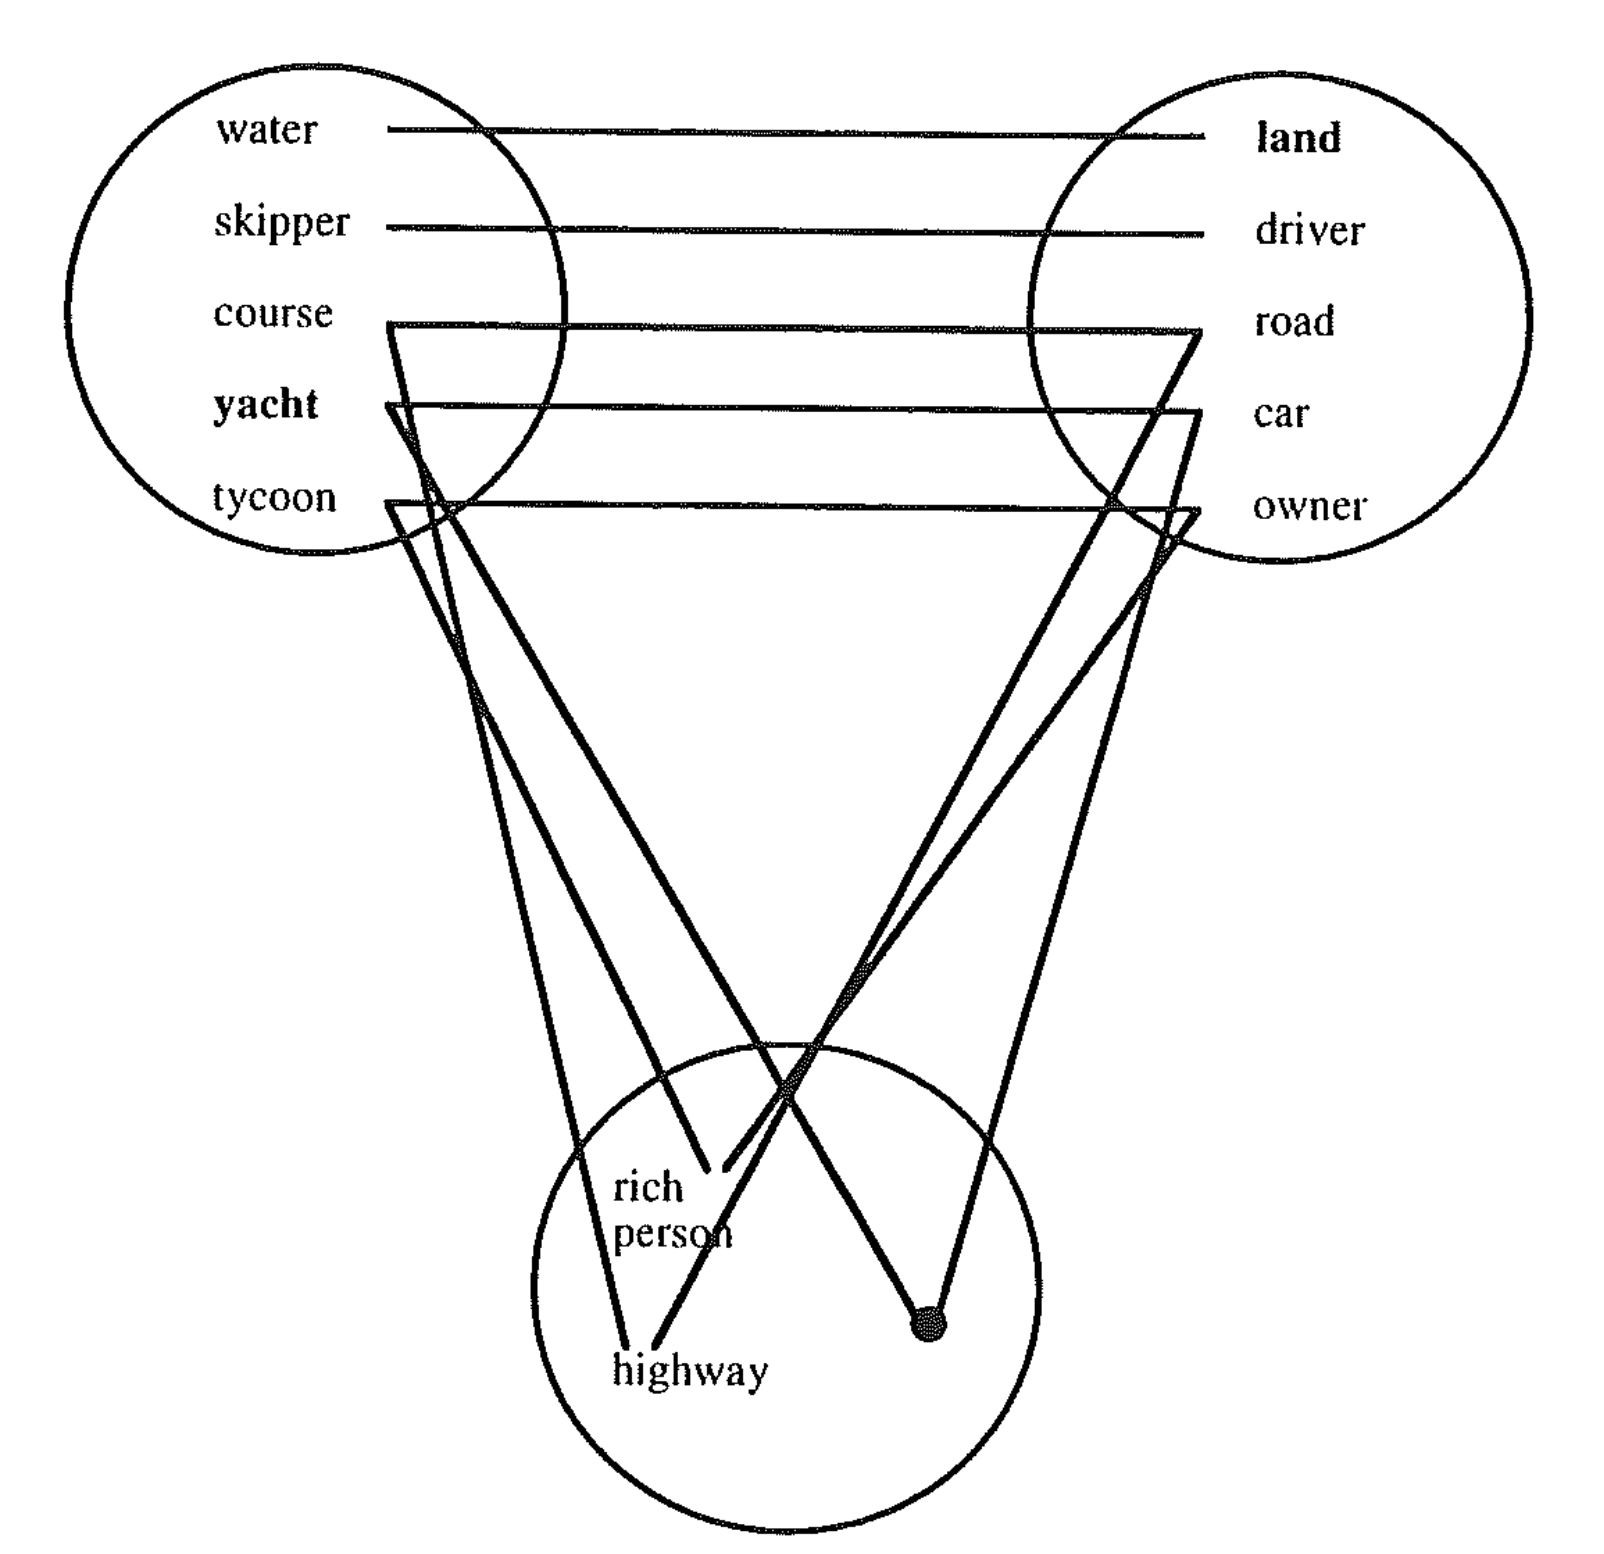
\includegraphics[width=0.8\textwidth]{figures/landYacht.png}
    \caption[Land yacht conceptual blend]{The conceptual blend of a \textit{land
            yacht}\footnotemark}\label{fig:landYacht}
\end{figure}

\footnotetext{Diagram borrowed from \citeauthor{conceptBlending},~\cite[67]{conceptBlending}.}

We note how this is how \acrshortpl{llm} operate when processing vectorized
linguistic data.
% Conceptual blending is a theory on both machine and human intelligence. 


\subsection{Utilising \acrshortpl{llm} - Prompt engineering}\label{sec:llmUtilization}


A typical way of interacting with \acrshortpl{llm} is \textit{prompting}~\cite[44]{llmSurvey}. You
prompt the model to solve various tasks. As we saw in \Nref{sec:emergentAbilities}, the level of
performance you are able to extract from your \acrlong{llm} can depend a great deal on how you
interact with it. The process of manually creating a suitable prompt is called \textbf{prompt
    engineering}~\cite[44]{llmSurvey}.~\citeauthor{llmSurvey} outline three principal prompting
approaches:

\textbf{\acrfull{icl}} is a representative prompting method that formulates the task
description and/or demonstrations in natural language text~\cite[44]{llmSurvey}. It is based on
\textit{tuning-free prompting} and it, as the name implies, never tunes the parameters of the
\acrshort{llm}~\cite[15]{promptingSurvey}. One the one hand, this allows for efficiency, but on the
other hand, heavy engineering is typically required to achieve high accuracy, meaning you must
provide the \acrshort{llm} with several answered prompts~\cite[16]{promptingSurvey}. In layman's
terms, \acrshort{icl} entails including examples of the process you want the model to perform when
prompting it.

\textbf{\acrfull{cot} prompting} is proposed to enhance \acrlong{icl} by involving a
series of intermediate reasoning steps in prompts~\cite[44, 52]{llmSurvey}. The basic concept of
\acrshort{cot} prompting, is including an actual \acrlong{cot} inside the prompt that shows the way
form the input to the output~\cite[52]{llmSurvey}.~\citeauthor{llmSurvey} note that the same effect
can be achieved by including simple instructions like `\textit{Let's think step by step}' and other
similar `magic prompts' in the prompt to the \acrshort{llm}, making \acrshort{cot} prompting easy to
use~\cite[52]{llmSurvey}.

\textbf{Planning} is proposed for solving complex tasks, which first breaks them down into smaller
sub-tasks and then generates a plan of action to solve the sub-tasks one by
one~\cite[44, 54]{llmSurvey}. The plans are being generated by the \acrshort{llm} itself upon
prompting it, and there is a distinction between text-based and code-based approaches. Text-based
approaches utilise natural language, whereas code-based approaches utilise executable computer code~\cite[54-55]{llmSurvey}.


\subsection{General challenges with \acrshortpl{llm}}\label{sec:llmProblems}

We have seen that \acrshortpl{llm} demonstrate promising abilities (\Nref{sec:emergentAbilities}) But they have nevertheless certain issues attached to them that we need to be aware of.

\subsubsection{Hallucination}\label{sec:llmHallucination}

As we saw in \Cref{sec:llmParrot}, \acrshortpl{llm} are prone to
\textit{bullshitting}. They have no intuition of, or concern with \textit{the
    truth}. They only ever yield whatever response is the most probable under their
\textsc{beam search} algorithm being applied on their training data.

\subsubsection{Environmental concerns}

A University of Rhode Island study on the environmental impact of \acrshortpl{llm} have shown that
they require wast amount of energy and water~\cite{hungryLlm}. They also found that the different
\acrshortpl{llm} may differ greatly in their energy consumption, highlighting that that certain
\acrshortpl{llm} may consume more than \num{70} times more energy than others~\cite{hungryLlm}.

Another study by \citeauthor{llmCarbon} focusing specifically on \textit{carbon emissions} did
however find that these emissions significantly lower for \acrshortpl{llm} than humans for specific
tasks such as text and image generation, ranging from \num{130} to \num{2900} times less Co2 emitted
depending on the task~\cite[1]{llmCarbon}.

\citeauthor{thirstyLlm} surveyed the water consumption of \acrshortpl{llm}, finding that training the
\acrshort{llm} \textsc{GPT-3} could evaporate as much as \num{700000} litres of clean
freshwater~\cite[1]{thirstyLlm}. Furthermore they review the trends of current AI adoption and
project that the water consumption of AI could reach levels as high as \num{4.2} - \num{6.6} billion
cubic metres by \num{2027}, which is comparable to \num{4} - \num{6} Denmarks, or half of the United
Kingdom~\cite[1]{thirstyLlm}. Recent research indicates that \textit{serving} \acrshortpl{llm}
currently account for more emissions than training them~\cite[37]{sustainableLlmServing}.

Efforts to achieve greener \acrshortpl{llm} have been proposed by \citeauthor{sproutGreenLlm}, while
recognizing the trade-off between ecological sustainability and high-quality
outputs~\cite[21799]{sproutGreenLlm}.

% TODO: Include or not?
% \subsubsection{Cognitive atrophy}
% https://arxiv.org/abs/2506.08872 

% TODO: Include or not?
% \subsubsection{LLM collapse}
% https://machinelearning.apple.com/research/illusion-of-thinking 


\subsection{The different kinds of \acrshortpl{llm}}\label{sec:llmJungle}

There are several available \acrshortpl{llm}, some of which are open source, and some proprietary.
Open source \acrshortpl{llm} afford greater insight into their composition and underlying training
data, whereas proprietary models appear more like black boxes. Some popular model families include
the GPTs, Gemini, Llama, Claude, Mistral, and DeepSeek.

The \acrshortpl{llm} differ primarily in their \begin{inparaenum}
    \item parameters, and
    \item training data.
\end{inparaenum}
As we saw in \Cref{sec:llmArch}, all typical \acrshortpl{llm} utilise a transformer-based neural
network. But due to their various different properties, different models can behave differently for
different tasks regardless of their similar architecture.

What they all share is their ability to perform \textit{inference}, meaning that they predict output
tokens given some input tokens (see \Cref{sec:llmParrot}).

\subsection{Existing \acrshort{llm} applications for \acrshortpl{ads}}\label{sec:llmsForAds}


\citeauthor{LLM4AD} give a broad overview of some of the ways \acrshortpl{llm} have been applied for
\acrshortpl{ads}, highlighting some of the opportunities and potential weaknesses of \acrshort{llm}
applications for \acrshort{ads} purposes. One of the ways \acrshortpl{llm} can be applied, is for
adjusting the driving mode, or aiding in the decision-making
process~\cite[1]{LLM4AD}.~\citeauthor{driveAsYouSpeak} delve further into these aspects in their
other work \citetitle{driveAsYouSpeak}, providing a framework for integrating \acrlong{llm}'s
\begin{inparaenum}
    \item natural language capabilities,
    \item contextual understanding,
    \item specialized tool usage,
    \item synergizing reasoning, and
    \item acting with various modules of the \acrshort{ads}
\end{inparaenum}~\cite[1]{driveAsYouSpeak}.
\chapter{Related work}\label{sec:relatedWork}

\section{DeepScenario}\label{sec:deepScenario}

DeepScenario is both a dataset and a toolset aimed at \acrlong{ads} testing~\cite{DeepScenario}. The
principal value proposition of this work lies in recognizing the fact that \begin{inparaenum}
  \item there are an infinite number of possible driving scenarios, and
  \item generating critical driving scenarios is very costly with regard to time costs and
  computational resources\end{inparaenum}~\cite[52]{DeepScenario}. The authors therefore propose
an open driving scenario of more than \num{30000} driving scenarios focusing on \acrshort{ads}
testing~\cite[52]{DeepScenario}. The project utilises traditional machine learning
methodologies, having been performed prior to the broad adaptation of \acrshortpl{llm}.

Its scenarios are intended for the simulator SVL by LG (\Cref{sec:simulatorOverview}).

\section{RTCM}

RTCM is a \acrshort{ads} testing framework that allows the user to utilise natural language for
synthesizing test cases. The authors propose a domain-specific language --- called RTCM, after
\textsc{Restricted Test Case Modelling} --- for specifying test cases. It is based on natural language
and composed of \begin{inparaenum}
  \item an easy-to-use template,
  \item a set of restriction rules, and
  \item keywords \end{inparaenum}~\cite[397]{RTCM}.  Furthermore, they also propose a tool to
take this RTCM source code as input and generating either \begin{inparaenum}
  \item manual, or
  \item automatically \end{inparaenum} executable test cases~\cite[397]{RTCM}. The proposed tools
were evaluated in experiments with industry partners, successfully generating executable test
cases~\cite[397]{RTCM}.

\section{DeepCollision}

\citeauthor{deepCollision} utilise \acrfull{rl} for \acrshort{ads} testing, with the goal of getting
the \acrshort{ads} to \textit{collide}. They used \textit{collision probability} for the loss
function of the \acrlong{rl} algorithm~\cite[384]{deepCollision}. Their experiments included
training 4 DeepCollision models, then using \begin{inparaenum}
  \item random, and
  \item greedy
\end{inparaenum} models for generating a baseline to compare their models with. The results showed
that DeepCollision demonstrated significantly better effectiveness in obtaining collisions than the
baselines. While not specifically focused on \textit{testing}, we recognize that their work is thematically
similar to our envisioned project.

\section{AutoSceneGen}

AutoSceneGen is a framework for \acrshort{ads} testing using \acrshortpl{llm},
focusing on the motion planning of \acrlong{ads}~\cite[14539]{autoSceneGen}.
\citeauthor{autoSceneGen} highlights how \acrshortpl{llm} provide opportunities
for efficiently evaluating \acrshort{ads} in a cost-effective
manner~\cite[14539-14540]{autoSceneGen}. They generate a substantial set of synthetic scenarios and
experiment with using \begin{inparaenum}
  \item only synthetic data,
  \item only real-world data, and
  \item a combination of the \num{2} \end{inparaenum} as training data. They find that motion
planners trained with their synthetic data significantly outperforms those trained solely on
real-world data~\cite[14539]{autoSceneGen}.

\section{LLM4AD}

LLM4AD is a paper that gives a broad overview of \acrshortpl{llm} for \acrlong{ads}. It touches on
several of the various \acrshort{ads} applications where \acrshortpl{llm} are relevant such as
\begin{inparaenum}
  \item language interaction,
  \item contextual understanding,
  \item zero-shot and few shot planning allowing \acrshortpl{llm} to perform tasks they weren't trained
  on, helping with handling edge cases
  \item continuous learning and personalization, and finally
  \item interpretability and trust \end{inparaenum}~\cite[2]{LLM4AD}. Furthermore, the authors
also propose a comprehensive benchmark for evaluating the instruction-following abilities of an
\acrshort{llm} based system in \acrshort{ads} simulation~\cite[1]{LLM4AD}.

\section{LLM-Driven testing of \acrshort{ads}}

\citeauthor{LLMDrivenTestingADS24} worked on using \acrshortpl{llm} to for automated test generation
based on free-form textual descriptions in the area of automotive~\cite[173]{LLMDrivenTestingADS24}.
They propose a prototype for this purpose and evaluate their proposal for \acrshort{ads} driving
feature scenarios in Carla. They used the \acrshortpl{llm} GPT-4 and Llama3, finding GPT-4 to
outperform Llama3 for the stated purpose. Their findings include this \acrshort{llm}-powered test
methodology to be more than \num{10} times faster than traditional methodologies while reducing
cognitive load~\cite[173]{LLMDrivenTestingADS24}.
% TODO: Cognitive load -> brain atrophy (sec:llMproblems)

\section{Requirements All You Need?}

\citeauthor{requirementsAllYouNeed} provide an overview of \acrshortpl{llm} for \acrshort{ads} in
their recent preprint~\citetitle{requirementsAllYouNeed}\footnote{This was submitted to Arxiv on
  2025-05-19.}, focusing on \acrshort{llm}'s abilities for translating abstract requirements extracted
from automotive standards and documents into configuration for Carla (\Cref{sec:simulatorOverview})
simulations~\cite{requirementsAllYouNeed}. Their experiments include employing the
\textit{autonomous emergency braking} system and the sensors of the \acrshort{ads}. Furthermore, they
split the requirements into \num{3} categories: \begin{inparaenum}
  \item vehicle descriptions,
  \item test case pre-conditions, and
  \item test case post-conditions (\Nref{sec:testingConditions})
\end{inparaenum}~\cite{requirementsAllYouNeed}. The preconditions they used included
\begin{inparaenum}
  \item agent placement,
  \item desired agent behaviour, and
  \item weather conditions amongst others\end{inparaenum}, whereas their postconditions reflected
the desired outcomes of the tests, primarily related to the vehicle's
telemetry~\cite{requirementsAllYouNeed}.

\section{Language Conditioned Traffic Generation}

\citeauthor{languageconditionedtrafficgeneration} look into using \acrshortpl{llm} to generate
specific traffic scenarios. They identify the importance of being able to use simulators to test
\acrshortpl{ads}, and highlight how test scenarios are expensieve to
obtain~\cite[1]{languageconditionedtrafficgeneration}. To this end, they propose a tool --
\textsc{LTCGen} which employs the strengths of \acrshortpl{llm} to match a natural language query
with a fitting underlying map\footnote{Map as in a \textit{world} in which a scenario can take
  place.}, and populates this with a \begin{inparaenum}
  \item initial traffic distribiution, and
  \item the dynamics of all the vehicles involved in the scene.
\end{inparaenum}
Something to note is that they generate their scenarios, without initially taking the \textit{ego
  vehicle} into account. The ego vehicle of the scene is simply determined as the vehicle that is
in the \textit{center} of the first
\textit{frame}~\cite[3]{languageconditionedtrafficgeneration}.

\section{Chat2Scenario}

\citeauthor{chat2Scenario} propose a method for utilising \acrshortpl{llm} to retrieve
\acrshort{ads} scenarios given a natural language query. Their framework synthesizes scenarios from
naturalistic\footnote{Their term. The intended meaning of \textit{naturalistic} is not all clar to
  me.} driving datasets, based on observation real world human driving~\cite[55]{chat2Scenario}, that
it then uses as a database for retrieveing the scenario that best matches the user's natural
language query. Furthermore, they employ traditional techniques for asserting the relevance of the
retrieved scenarios, allowing the user to specify a set of \textit{criticality metrics}, of which a
certain threshold must be reached amongst the scenarios that are initalliy retried by the
\acrshort{llm}, pruning false positives. As a measure to increase the usability of their framework,
they also provide a webapp with an intuitive \acrshort{gui} for both \begin{inparaenum}
  \item operating the tool, and
  \item visualizing the scenarios \end{inparaenum}~\cite[560]{chat2Scenario}.

In order to allow the \acrshort{llm} to determine whether a scenario is relevant under the
provided query, they put forward a method for classifying the various scenarios using traditional
\acrshort{ml} techniques. This classification focuses primarily on highway scenarios and the
activities of other actors in relation to the ego vehicle~\cite[561-562]{chat2Scenario}.

\subsubsection*{Prompt engineering}

% TODO: Legge inn kryssreferanse til background om prompt engineering? 

The project's prompts are `informed' by the \num{6} \acrlong{oai} guidelines from their prompt
engineering guide\footnote{\url{https://platform.openai.com/docs/guides/prompt-engineering} (URL
  from the paper.)}, ending up with a structured prompt of \num{5} segments. These segments serve to
guide the \acrshort{llm}, delineating its role as an `advanced \acrshort{ai} tool for scenario
analysis, specifically tasked with interpreting driving scenario following a pre-established
classification model'~\cite[562]{chat2Scenario}. They then input the user-provided description of
the scenario they wish to retrieve. Following this, a third segment declares the format for the
\acrshort{llm} response, followed by a prime example of \acrlong{icl}, demonstrating what a
satisfactory fulfillment of the desired format could look like. Lastly they instruct the
\acrshort{llm} to \textit{Remember to analyze carefully and provide the classification as per the
  structure given above}~\cite[563]{chat2Scenario}.
% TODO: Ref siste punkt om "husk å gjøre det riktig" -> kan skrive om dette fenomenet i background
% og så referere tilbake til det.

\chapter{Proposed solution and implementation details}\label{sec:solutionProposal}

\epigraph{Do or do not, there is no try}{Master Yoda}

\section*{Pitch}

We have seen that \acrshort{ads} testing is \textit{complex} and that it is difficult to get a good
test coverage (\Cref{sec:adsTestingComplexity}). Furthermore, we have seen that \acrshortpl{llm}
have \textit{emergent abilities} (\Cref{sec:emergentAbilities}). We therefore propose a tool for
\begin{inparaenum}
    \item running a base \acrshort{ads} test case,
    \item enhancing the test case using \acrshortpl{llm},
    \item running the enhanced test case, and
    \item comparing the results of the two runs.
\end{inparaenum}

This will allow us to learn the extent to which \acrshortpl{llm} can be applied for enhancing
\acrlong{ads} test cases. We will survey several \acrshortpl{llm} and evaluate their applicability
for the problem at hand, in light of what we know about \acrshortpl{llm} (\Nref{sec:llmJungle}). We
want to have a pipeline that is able to process several test cases in succession, in order to get a
substantial dataset.

Let the pipeline tool be known as \hefe.~%\info{This name is naturally just a placeholder.}.
The tool follows a natural pipeline structure. We have some base test cases that
need to be ran in order to get a baseline for the results, we then have to
improve these, and run the improved versions and compare them to their original
versions. The architecture of the tool is visualised in \Cref{fig:hefeArch}.

\begin{figure}[h]
    \centering
    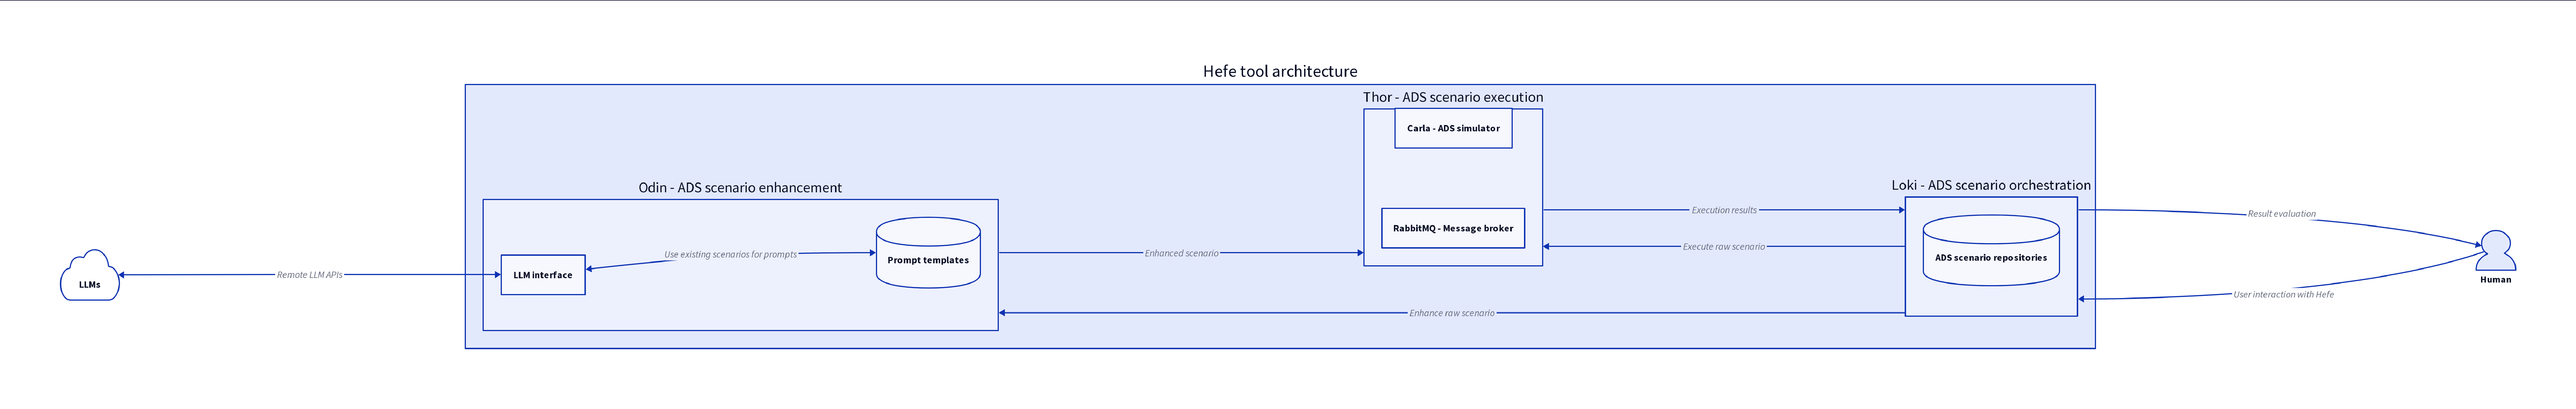
\includegraphics[width=\textwidth]{figures/d2-pdf/hefe.pdf}
    \caption{\hefe~pipeline architecture}\label{fig:hefeArch}
\end{figure}


Furthermore, as outlined in \citeauthor{LLM4AD}, \acrlongpl{llm} can be applied to several aspects
of \acrlong{ads}. It is not feasible that we focus on \textit{all} these aspects, and as such we
should narrow down our scope. Let us review some of the relevant aspects.

% Vi vil fokusere på driveability

% \section*{The applicability of \acrshortpl{llm} in \acrshort{ads} testing}
\section{Broad architectual overview}


\acrlong{ads} are typically modular, as we have seen in \Cref{sec:adsTestingComplexity}.
\acrshortpl{llm} are applicable to the different modules in different ways as we saw in
\Nref{sec:relatedWork}.
% TODO: Make more specific reference to what part of Related Work

\begin{tcolorbox}[colback=gray!5!white,colframe=gray!75!black,title=User history
        of using \hefe]\label{user-history}
    I have a set of \acrfull{ads} test cases. I provide this set to \hefe. It will run the entire
    set, and generate a baseline of my \acrshort{ads} performance.

    \hefe~will then improve my test cases using \acrlongpl{llm} and run them again.

    Lastly \hefe~will report how the results differ from running the base and enhanced version of a
    test case.

    This will give me insight into what caused my \acrshort{ads} to fail so that I can look into the
    cause of the error state and uncover underlying faults in the \acrlong{ads}.

\end{tcolorbox}


\subsection{Implementation language}

The programming language \textsc{Python} is widely used for \acrfull{ads} simulation. It is a high
level language, allowing the user great flexibility and developer experience. For this reason, I will
implement \hefe~using Python.

Python can be optimized using \acrfull{jit} compilers such as Numba~\cite{numba}, which can speed up
our execution times. Libraries such as Joblib provide Python with plug-and-play
meomization, which will allow us to re-use values that have already been
computed, saving time and energy.


\subsection{Overview of the components of the \hefe~pipeline}

The pipeline architecture is visualised in \Nref{fig:hefeArch}. Here we
present the major components and their responsibilities


\subsubsection{Test case enhancement}

\subsubsection{Test case repositories}

We have seen in \Nref{sec:relatedWork} that there are existing repositories of
% TODO: Make more specific reference to what part of Related Work
\acrshort{ads} test cases. These will provide us with \begin{inparaenum}
    \item a baseline,
    and
    \item data onto which we can apply our \acrshort{llm} enhancements.
\end{inparaenum}

\subsubsection{\acrshort{llm} enhancement}\label{sec:llmEnhancement}
% TODO: Dette må spisses mot driveability

The base test cases will individually be enhanced by prompting the
\acrshort{llm}. We will experiment with several \acrshortpl{llm}.

For performing the actual improvement, it is essential that we \begin{inparaenum}
    \item test several \acrshort{llm},
    \item give clear prompts
    % \info{I'm inclined to find some fitting prompts through trial and error, as such a I do not wish to describe them in detail at this time.}
    and
    \item verify that the returned test case adheres to the strictly necessary
    syntax rules. This last point is important due to our knowledge of
    \acrshortpl{llm} hallucinating (see \Nref{sec:llmProblems}).
    % TODO: More specific reference to Halucination intead of all LLm problems?
\end{inparaenum}

In order to facilitate testing various \acrlongpl{llm}, we should employ
\acrshort{llm} agnostic software as a translation layer. This will allow us to
write code for a common interface and test several \acrshortpl{llm} that may all
have different internal \acrfullpl{api} without having to modify our test code
for specific \acrshortpl{api}. This \begin{inparaenum}
    \item saves time
    and
    \item makes for more even test conditions \end{inparaenum}. Some pieces of software providing
this type of functionality include
\textsc{aisuite}\footnote{\url{https://github.com/andrewyng/aisuite}}, RamaLama from
RedHat\footnote{\url{https://github.com/containers/ramalama}}, and the MIT licensed
Ollama\footnote{\url{https://github.com/ollama/ollama}}, both supporting a plethora of
\acrlongpl{llm}.

\textsc{guidance}\footnote{\url{https://github.com/guidance-ai/guidance}} is a
framework for limiting the room in which \acrshortpl{llm} may operate, which
might be useful if we run into issues with excessive hallucination.


\subsubsection{Enhanced test case validation}

We must expect the \acrshort{llm} to hallucinate to some extent (\Cref{sec:llmHallucination}). We
therefore propose to verify the format of the enhanced file before running it.

As we saw in the section for \Nref{sec:adsScenarioFormats}, there exists several formats for
\acrshort{ads} scenarios. In order to verify that the syntax of our enhanced test
case is valid, we simply need to apply the syntax rules of our format.

The CommonRoad format is XML-based~\cite[720]{commonRoadOG} and as such we can
to some extent assess the degree of hallucination by parsing the XML structure.
Furthermore, it has an exhaustive Python library with several utilities\footnote{\url{https://pypi.org/user/commonroad/}}.

OpenSCENARIO exists both as XML and a domain-specific language (DSL). If we
utilise the XML version, we can apply the same methodology as for the CommonRoad
format. If using the DSL version, one way
the OpenSCENARIO format can be verified is by using free
online cloud services such as this offering from AVL
\footnote{\url{https://smc.app.avl.com/validation}}. We should however strive for
running a local verification service to \begin{inparaenum}
    \item save time and compute,
    and
    \item preserve data privacy.
\end{inparaenum}
Besides, it is generally a good idea to limit the number of external dependencies\footnote{Note for
    example how LGSVL\cite{lgsvl} was shut down, preventing projects such as DeepScenario of
    \citeauthor{DeepScenario} to be further developed on the original platform.}.

\subsection{Test case running and evaluation}

\subsubsection{Test case runner}

The system will automatically run all
our base test cases using an \acrshort{ads} simulator, and collect data points to get a baseline. It
will later also run the mutated \acrshort{llm}-enhanced versions of the base cases.

We have already ran the test cases in their base form. We will now run their
improved versions in order to compare them to see what effect the \acrshort{llm}
enhancement (see \Cref{sec:llmEnhancement}) has had.

For the reasons we have seen in~\Cref{sec:simulatorOverview}, we want to run our
test cases on Carla. It is the best offering as it is open source, under active
development and has a feature rich Python \acrshort{api}.

\subsubsection{Test case improvement evaluation}\label{sec:testCaseEval}

We saw in \Cref{sec:adsMetrics} that there are several metrics for assessing
\acrshort{ads}. We will use these metrics when evaluating our improvements.

\subsubsection{Test case result reporting}

We will compare the results from running
the baseline unmodified test case and comparing it with the results from
running the \acrshort{llm}-enhanced version and returning to the user. Ideally with
some automatic analysis of the results.

Having ran both the base test case and its enhanced counterpart, we have
results. The results will be stored in \acrfull{csv} files, allowing \begin{inparaenum}
    \item further analysis in Python/Jupyter,
    and
    \item easy translation to \LaTeX tables for the final report.
\end{inparaenum}

This is the final step of the envisioned pipeline. Where we have our result, and
need to analyse them.

This last step has great opportunities for being scoped up to a fully integrated
test suite which allows for both running test cases and analysing the results in
a \acrfull{gui}. But we should focus on the prior steps for now, only creating a
\acrshort{gui} if there is sufficient time towards the end of the project to
focus on such non-\acrshort{llm} related topics.

Initially, the results will consist of numerical comparison of the
\acrshort{csv}s with regard to the relevant metrics outlined in
\Nref{sec:testCaseEval}.

We need to define what requirement we will use for determining the \textit{result} of a test case
run. Without this, we cannot compare it to other test cases.

\section{Component details}

Having begotten a broad overview of the details of the \hefe pipeline, let us now narrow our scope
and focus on the individual components.

% Alt under her er kopiert over fra det gamle "implementation details"-chpt.
% (Og så tilpasset litt, dekrementert heading levels osv )


The implementation is what facilitates doing the actual experiments. For the
most part, it follows what is outlined in the \Nref{sec:solutionProposal}, with
some minor practical differences.
What follows will analyze the impelementation of the components of the \hefe{}
pipeline and explain more closely in detail not only \emph{what} they do, as
that is already covered in the solution proposal, but \emph{how} they do it, with
hands-on code examples.

% TODO: Burde avklare om den skal leve her "for alltid". Syns det kan gi emning
% å samle alle master ting i ett repo. Fortrinnsvis _dette_ (veldig meta å linke
% til seg selv i så fall hehe). Kan også være gunstig mtp å inkludere kode som appendix?
All code is available on the Github repo \href{https://github.com/orjahren/master-hefe}{\texttt{master-hefe}}.

\subsection{Carla interface and scenario utilities -- Thor}

The Thor module is responsible for all thigs related to the Carla \acrshort{ads}
simulator. It provides the client with several scenario-related utilities, and
is capable of executing the desired scenarios.


Certain of its utilities are simple tools for asserting the liveness of Carla,
such as the \texttt{get\_carla\_is\_up} function, shown in
listing~\ref{lst:odinCarlaHealthCheck}. This function will use the Caral
standard Python library and attempt to connect to the server on its default
port\footnote{I.e. \num{2000}, line \#4 in listing
    \ref{lst:odinCarlaHealthCheck}.}. Note that we refer to the host as simpyly
\texttt{carla} -- this is possible due to the entire project running
containerised with Docker Compose. Instead of refering to the speicifc IP
address of the Carla server (typically localhost, if not running it externally),
the Docker system will facilitate this name translation for us.

\begin{lstlisting}[caption={Exerpt from carla\_interface.py, demonstrating the implementation of a Carla health check.}, label={lst:odinCarlaHealthCheck}, language={Python}]
import carla

CARLA_HOST = "carla"
CARLA_PORT = 2000


def get_carla_is_up() -> bool:
    """
    Check if the CARLA simulator is up and running.
    This function attempts to connect to the CARLA server and returns True if successful, otherwise False.
    """
    print("Running carla integration check to see if it is up...")
    try:
        client = carla.Client(CARLA_HOST, CARLA_PORT)
        client.get_world()
        return True
    except Exception as e:
        print(f"CARLA connection failed: {e}")
        return False
\end{lstlisting}

This is used both to assert the general liveness of the \hefe pipeline, and to
verify that the simulator is available before performing experiments. It is
better to detect this illegal state \emph{before} running experiments rather
than during their execution.

Furthermore, it shall also be equipped with funcitonality for \emph{executing} \acrshort{ads}
scenarios on Carla. This is trivial when using Carla's existing Scenario Runner
module's funcitonality. As of now, this has not yet been implemented due to
greater challenges in the \acrshort{llm} module -- Odin.


% Rest API - running test cases - Thor
% “Fast API”, Python
% POST a test case to the API. It will be ran on the ‘server’
% RabbitMQ for listening for finished test cases? So that the client knows it can fetch the results?
% Will need UUID for test cases so the correct result can be fetched after it has been ran
% Need to store these somewhere. NoSQL database?
% This component should also accumulate results.
% Huge TODO: What metric are these results?
% Should be containerised (Docker/Podman)

\subsection{LLM interface and prompt applications -- Odin}\label{sec:odinImplementation}

% Rest API - performing LLM enhancement - Odin
% “Fast API”, Python
% Take a base test case as body
% Have some prompt repository
% Apply prompts with LLMs
% Must integrate with LLM. Either locally (Ollama) or remote (some API)
% Look into good LLM agnostic transition layer. E.g. Aisuite
% https://github.com/andrewyng/aisuite
% Should use same UUIDs as outlined above, but suffixed with e.g. “pure” and “tainted”
% Containerized. Docker compose?

The Odin module handles all things \acrshort{llm}. It provides a unified
\acrshort{api} for applying various prompts to scenarios and returning the
enhanced output resulting from having applied the prompt. We hve implemented
support for the \acrshortpl{llm} that are available on \begin{inparaenum}
    \item Ollama, and
    \item Gemini
\end{inparaenum}. This allows for testing with \acrshortpl{llm} such as
\begin{inparaenum}\setcounter{enumi}{2}
    \item Mistral \num{7.2}B, and
    \item gemini-2.5-flash
\end{inparaenum}.

\subsection*{LLM interface implementations}
\subsubsection{Gemini integration}

The Gemini integration is quite straightforward, relying on Google's own
\texttt{genai} Python module. Listing~\ref{lst:thorGeminiInterface} renders the
\emph{entire} interface, again highlighting how straightforward this really is.
The one piece of complexity to not is that it requires that the user provides
their own Gemini \acrshort{api} key and has this set as an environment variable
with the proper name. Without this being as it should, the script will crash, as
it would not possible for it to complete the desired \acrshort{llm} enhancement
regardless as long as the \acrshort{api} key is not present.

\begin{lstlisting}[caption={llm\_api\_interfaces/gemini\_interface.py, The implementation of a Gemini interface for executing prompts.}, label={lst:thorGeminiInterface}, language={Python}]
import os


from google import genai


def get_api_key() -> str:
    api_key = os.getenv("GEMINI_API_KEY")
    if not api_key:
        raise EnvironmentError("GEMINI_API_KEY environment variable not set.")
    return api_key


client = genai.Client(api_key=get_api_key())


def api_is_up():
    return True  # Assume Google never dies...


# TODO: Use decorator for asserting API liveness? Or standard assertion??
def execute_gemini_model(model_name: str, prompt: str) -> str:

    response = client.models.generate_content(
        model=model_name or "gemini-2.5-flash",
        contents=prompt
    )

    return response.text
\end{lstlisting}

\subsubsection{Ollama integration}

The Ollama integration is a bit more cumbersome. This motly comes down to it not
using any exisitng library modules for this specific purpose, instead relying on
using the \texttt{json} and \texttt{requests} modules to implement the desired
funcitonality from scratch, making it so that we need to handle network IO and
marshalling the \acrfull{llm} response into a fitting return buffer.

Listing~\ref{lst:thorOllamaInterface} renders the
\emph{entire} interface. As we can see, it is not too bad allthough nowhere near
as clean as the Gemini implementation (\ref{lst:thorGeminiInterface}).

Its complexity arises principally from \num{2} major factors --
\begin{inparaenum}
    \item the already mentioned manual networking, and
    \item having to parse the streamed response
\end{inparaenum}
Furthermore, this code expects that the user already \emph{has} an Ollama
installation running on their host machine. The code provides no means of setup
for this -- that is an entirely external endeavour that is left up to the end user.

Similarly to how the Gemini implementation does it, this will crash if Ollama is
not funcitoning properly as it would not possible for it to complete the desired
\acrshort{llm} enhancement regardless if Ollama is unreachable.

\begin{lstlisting}[caption={llm\_api\_interfaces/ollama.py, The implementation of an Ollama interface for executing prompts.}, label={lst:thorOllamaInterface}, language={Python}]
import json
import requests


OLLAMA_API_URL = "http://localhost:11434"


def api_is_up():
    try:
        response = requests.get(OLLAMA_API_URL)
        return response.status_code == 200
    except requests.ConnectionError:
        return False


# ollama models
def get_ollama_models():
    try:
        response = requests.get(f"{OLLAMA_API_URL}/api/tags")
        if response.status_code == 200:
            return response.json()["models"]
        else:
            print(f"Failed to get models: {response.status_code}")
            return []
    except requests.ConnectionError:
        print("Failed to connect to the API.")
        return []


# TODO: Use decorator for asserting API liveness? Or standard assertion??
def execute_ollama_model(model_name: str, prompt: str):
    try:
        payload = {
            "model": model_name,
            "prompt": prompt
        }
        print(f"Executing model {model_name} with prompt: {prompt}")
        response = requests.post(
            f"{OLLAMA_API_URL}/api/generate", json=payload)
        if response.status_code == 200:
            result = ""
            for line in response.iter_lines():
                if line:
                    data = line.decode('utf-8')
                    try:
                        json_obj = json.loads(data)
                        result += json_obj.get("response", "")
                    except Exception as e:
                        print(f"Failed to parse line: {e}")
            return {"text": result}
        else:
            print(f"Failed to execute model: {response.status_code}")
            return None
    except requests.ConnectionError:
        print("Failed to connect to the API.")
        return None
\end{lstlisting}

\subsection*{Prompts and their associated code}

In this project, the prompts are the instruction to the \acrfull{llm} for
applying the enhancement to the scenario. Quite possibly the most critical piece
of code related to the experiments. They need to take the base scenario as an
input and integrate it into the \acrshort{llm} context, such that it knows what
it shall use as its base to apply enhancements that will decrease the
driveability. For this reason, it also provides certain scenario
utilities\footnote{That architectually might as well have been integrated in the
    Thor module\ldots}.

\subsubsection{Scenario utilities}

These are essentially quite trivial helpers. Lisitng \ref{lst:odinScenarioUtils}
render the core functionality -- hopefully this is quite self-explaining.

\begin{lstlisting}[caption={scenario\_utils.py, The implementation of an various scenaro helper functions for executing prompts.}, label={lst:odinScenarioUtils}, language={Python}]
import os


# TODO: Implementer denne
# TODO: Fastslaa hvilket format vi bruker (OpenSCENARIO/CommonRoad/andre)
def file_format_is_valid(file_format: str) -> bool:
    """
    Check if the file format is valid.

    Args:
        file_format (str): The file format to check.

    Returns:
        bool: True if the file format is valid, False otherwise.
    """
    return file_format in ["json", "yaml", "yml", "csv", "txt"]


def enumerate_enhanced_scenarios(scenario_repository_path: str, scenario_name: str) -> int:
    """
    Enumerate enhanced scenarios in a given scenario path.

    Args:
        scenario_repository_path (str): The path to the scenario directory.
        scenario_name (str): The name of the scenario.

    Returns:
        int: The number of enhanced scenarios found.
    """
    # TODO: Can probably refactor this
    acc = 0
    for scenario in os.listdir(scenario_repository_path):
        print(f"Checking scenario: {scenario}")
        if scenario_name in scenario and "enhanced" in scenario:
            acc += 1
    return acc


# TODO: Should use better names. Need a way of tracking enhanced scenario
# metadata
# - Timestamp
# - What prompt was used
# - What model was used
# - What the original scenario was
# - What changes were made?
def get_enhanced_scenario_name(scenario_repository_path: str, scenario_name: str) -> str:
    """
    Get the enhanced scenario name.

    Args:
        scenario_repository_path (str): The path to the scenario directory.
        scenario_name (str): The base name of the scenario.

    Returns:
        str: The enhanced scenario name.
    """
    num_enhanced_scenarios = enumerate_enhanced_scenarios(
        scenario_repository_path, scenario_name)
    if num_enhanced_scenarios == 0:
        return f"{scenario_name}-enhanced"
    else:
        # Big brain time...who needs UUIDs when you can just count files?
        return f"{scenario_name}-enhanced-{num_enhanced_scenarios + 1}"


def get_available_scenarios(scenario_repository_path: str) -> list:
    def extension_is_ok(filename: str) -> bool:
        # TODO: Verify which formats we want to support
        return filename in ["xosc", "py"]

    return [filename for filename in os.listdir(scenario_repository_path) if extension_is_ok(filename)]


# TODO: Should strip newlines??
def scenario_path_to_string(scenario_path: str) -> str:
    with open(scenario_path, 'r') as file:
        return file.read()


# TODO: Let this function determine output file name?
def save_enhanced_scenario(scenario_str: str, output_path: str):
    with open(output_path, 'w') as file:
        file.write(scenario_str)
\end{lstlisting}

\subsubsection{Prompts -- templating and usage}

% TODO: Finnes det noe bigbrain måte å slippe å manuelt måtte referere ti llinjenummer?
As mentioned, the prompts need to include the scenarios \emph{in} them, so that
they are accessible to the \acrshort{llm}. How this is done, is rendered in
listing~\ref{lst:odinPromptTestbed}. The most interesting aspect is how the
prompts are stored in the system as lambda functions. This makes it so that they
can take an argument that represents the scenario --
\texttt{python\_carla\_scenario\_raw}(line \#16) -- and simply \emph{execute} the
function to insert the scenario into the prompt (line \#42). This is then
inserted into the output prompt at the location located at line \#21 in the listing.

\begin{lstlisting}[caption={experiments/testbed/prompts.py, The implementation of a prompt testbed for executing prompts.}, label={lst:odinPromptTestbed}, language={Python}]
# We wish to decrease the driveability of the scenario by enhancing it with more
# details, increasing its complexity

# Prompt structure:
"""
1 - Context: We are working with a driving simulation environment for the Carla simulator.
2 - Task: Decrease the driveability of the scenario by enhancing it with more details and complexity.
3 - Input: <scenario_description, in python carla scenario format>
4 - Output: An enhanced version of the scenario description with additional
details and complexity, still in Python carla scenario format. ONLY output the
code, without any additional text or explanation.
"""

PROMPTS = [
    [...] # NOTE: Removed most prompts from this listing for brevity.
    lambda python_carla_scenario_raw: f"""
    1 - Context: You are a tool for decreasing the driveability of scenarios in the driving simulator Carla.
    2 - Task: Decrease the driveability of the scenario by enhancing it with
    more details and complexity, using only methods that are part of the
    official Carla API, version 0.9.15.
    3 - Input, the Python specification for the scenario: {python_carla_scenario_raw}
    4 - Reasoning: Think step by step about how to make the scenario more complex and less driveable, considering possible obstacles, traffic, weather, and other factors using only the official Carla API.
    5 - Output: Only output the enhanced scenario code in Python Carla scenario format, with no additional text or explanation.
    """,
]


def name_to_prompt_idx(name: str) -> int:
    mapping = {
        "basic": 0,
        "no_explanation": 1,
        "no_explanation_strict": 2,
        "cot": 3,
        "cot_strict_methods_in_file": 4,
        "cot_strict_carla_api": 5,
    }
    return mapping.get(name, 0)


def get_prompt_for_python_scenario_enhancement(python_carla_scenario_raw: str, prompt_name: str) -> str:
    prompt_idx = name_to_prompt_idx(prompt_name)
    return PROMPTS[prompt_idx](python_carla_scenario_raw)

\end{lstlisting}

Lastly, note the comments in the top of the file, intended to give Github
Copilot increased understanding of the context, so that it can provide better
aid during programming.


\subsection{Execution tool / user oriented frontend -- Loki}

% Client - orchestrating the process - Loki
% Fetch available test cases from Thor? Select what/which are to be used
% Store results clientside? Separate database for this?

The final module of the \hefe pipeline is Loki -- it is simply a tool intended
to be used by the user for operating the process. It \begin{inparaenum}
    \item  says what scenarios are available to it (i.e. those that are eligble for
    being enhanced), and
    \item allows the user to select a prompt and
    \item execute that prompt to the scenario of their choosing.
\end{inparaenum}


\begin{lstlisting}[caption={loki/main.py, The implementation of the Loki script.}, label={lst:lokiMainImplementation}, language={Python}]
import pika
import requests

# from odin.server import ODIN_PORT
# from thor.server import THOR_PORT

ODIN_PORT = 4000
THOR_PORT = 6000


# TODO: Merge health checks into a single function?
def do_thor_health_check():
    try:
        res = requests.get(f"http://localhost:{THOR_PORT}/health")
    except requests.ConnectionError:
        print("Thor server is not running or unreachable.")
        exit(1)
    if res.status_code == 200:
        # parse json
        health_status = res.json().get("status", "unknown")
        if health_status == "healthy":
            print("Thor is healthy.")
        else:
            print(f"Thor health check failed.: {health_status}")
            exit(1)
    else:
        print("Thor health check failed.")
        exit(1)


def do_odin_health_check():
    try:
        res = requests.get(f"http://localhost:{ODIN_PORT}/health")
    except requests.ConnectionError:
        print("Odin server is not running or unreachable.")
        exit(1)
    if res.status_code == 200:
        health_status = res.json().get("status", "unknown")
        if health_status == "healthy":
            print("Odin is healthy.")
        else:
            print(f"Odin health check failed.: {health_status}")
            exit(1)
    else:
        print("Odin health check failed.")
        exit(1)


def run_test_case(test_case_id):
    print(f"Running test case: {test_case_id}")

    # Run test case on Loki
    result = requests.post(
        f"http://localhost:{THOR_PORT}/run_test_case",
        json={"test_case_id": test_case_id})
    if result.status_code != 200:
        print(f"Failed to run test case: {test_case_id}")
        return None
    print(f"Test case {test_case_id} executed successfully.")
    value = result.json().get("result", "No result found")
    return value


def get_enhanced_test_case(test_case_id):
    print(f"Enhancing test case: {test_case_id}")

    # Enhance test case on Odin
    result = requests.post(
        f"http://localhost:{ODIN_PORT}/enhance_test_case",
        json={"test_case_id": test_case_id})
    if result.status_code != 200:
        print(f"Failed to enhance test case: {test_case_id}")
        return None
    print(f"Test case {test_case_id} enhanced successfully.")
    value = result.json().get("result", "No result found")
    return value


def get_improvement(base_test_case, enhanced_test_case):
    # Simulate getting an improvement between two test cases
    # TODO: Implement actual logic to compare test cases
    return f"Improvement from {base_test_case} to {enhanced_test_case}"


def send_test_message(message):
    # TODO: Implement proper credentail handling.
    credentials = pika.PlainCredentials('user', 'pass')
    connection = pika.BlockingConnection(
        pika.ConnectionParameters('localhost', credentials=credentials))
    channel = connection.channel()
    channel.queue_declare(queue='test_queue')
    channel.basic_publish(exchange='', routing_key='test_queue', body=message)
    print(f"Sent message to RabbitMQ: {message}")
    connection.close()


if __name__ == "__main__":
    print("Loki is running...")

    do_thor_health_check()
    do_odin_health_check()

    send_test_message("Hello from Loki!")

    exit(0)
    test_case_id = "test_case_123"

    print("Starting test case execution...")
    base_result = run_test_case(test_case_id)
    print(f"Base result: {base_result}")

    enhanced_test_case = get_enhanced_test_case(test_case_id)

    enhanced_test_case_result = run_test_case(enhanced_test_case)
    print(
        f"Enhanced test case execution completed with result: {enhanced_test_case_result}")

    improvement = get_improvement(base_result, enhanced_test_case_result)
    print(f"Improvement: {improvement}")

    print("Loki execution finished.")

\end{lstlisting}


Listing~\ref{lst:lokiMainImplementation} renders the implementation of the
script. It relies on the Odin and Thor modules for all essential functionality,
which is in line with what is to be expected as this is simply a frontend client
to \emph{reach} them.

It is relies on the \texttt{requests} module for doing \acrfull{rpc} to the
other modules. There is also the outlines of a RabbitMQ implementation, which is
why \texttt{pika} is being imported. As of now, this is in non-functioning
alpha. Implementation of RabbitMQ message passing has not been prioritized as
there were, as mentioned, more important issues to focus on that would yield
better and more important results when resolved. This would maintain feature
parity with the \texttt{requests}-based approach.

\backmatter

\references

\end{document}
